% Soutenance — thème « strontium »
% Compiler avec :  latexmk soutenance.tex   (LuaLaTeX, cf. latexmkrc)
% Graphes de comparaison PA : python3 scripts/graphes_PA.py
\documentclass[aspectratio=169, 11pt]{beamer}
\usetheme{strontium}

\usepackage[french]{babel}
\usepackage{appendixnumberbeamer}   % les diapos de secours ne comptent pas dans le total
\usepackage{siunitx}
\usepackage{braket}
\usepackage{booktabs}
\sisetup{locale=FR}

% Dossiers où chercher les figures (on pointe vers ceux du manuscrit)
\graphicspath{
  {figures/}
  {../Manuscrit_these/appendix/images/}
  {../Manuscrit_these/Chapitres/Gas preparation and spin control/images/}
  {../Manuscrit_these/Chapitres/Ramsey interferometers on qudit/article Coherent Manip/}
  {../Manuscrit_these/Chapitres/Engineering highly entangled system of photoassociated 87Sr atoms/images/}
}

\title[Contrôle optique du \textsuperscript{87}Sr ultrafroid]{Contrôle optique du \textsuperscript{87}Sr ultrafroid}
\subtitle{Des manipulations de spin à un corps à la photoassociation de deux corps}
\author{Pauline Guesdon}
\date{Soutenance de thèse \textperiodcentered{} 14 décembre 2026}
\institute{Laboratoire de Physique des Lasers \textperiodcentered{} Université Sorbonne Paris Nord}
\renewcommand{\logostitre}{%
  
\includegraphics[height=0.75cm]{logo_USPN.png}\hspace{0.5cm}%
  
\includegraphics[height=0.75cm]{logo_ED_Galilee.png}}

% Cadre gris qui tient la place d'une figure : à remplacer par \includegraphics
\newcommand{\figurevide}[2]{%
  \tikz\node[draw=gris!50, dashed, fill=voile, minimum width=#1, minimum height=#2,
             text=gris, font=\small, align=center] {figure};}
% Note grise pour ce qui reste à compléter
\newcommand{\acompleter}[1]{{\color{gris}\small[#1]}}
\newcommand{\Sr}[1]{\textsuperscript{#1}Sr}

\begin{document}

% ---------------------------------------------------------------------
\begin{frame}[plain, noframenumbering]
  \titlepage
\end{frame}

\begin{frame}{Plan}
  \begin{enumerate}
    \item Introduction : le \Sr{87}, un atome à dix états de spin
    \item Manipulations cohérentes de pseudo-spins
    \item Photoassociation du \Sr{87}
    \item Conclusion et perspectives
  \end{enumerate}
\end{frame}

% =====================================================================
\section{Introduction}  % ~7 min : la motivation générale, pas de technique

\begin{frame}{Le \Sr{87} : un atome à dix états de spin}
  \begin{columns}[c]
    \begin{column}{0.46\textwidth}
      \begin{itemize}
        \item<1-> Spin nucléaire $I=9/2$ : \alert{10 états} $m_F$ dans le fondamental
        \item<2-> Fondamental $^1S_0$ ($J=0$) : \alert{faible sensibilité} au champ magnétique
        \item<3-> Raie étroite $^1S_0\to{}^3P_1$ (\SI{7.5}{kHz}) pour adresser chaque état
      \end{itemize}
    \end{column}
    \begin{column}{0.5\textwidth}
      \centering
      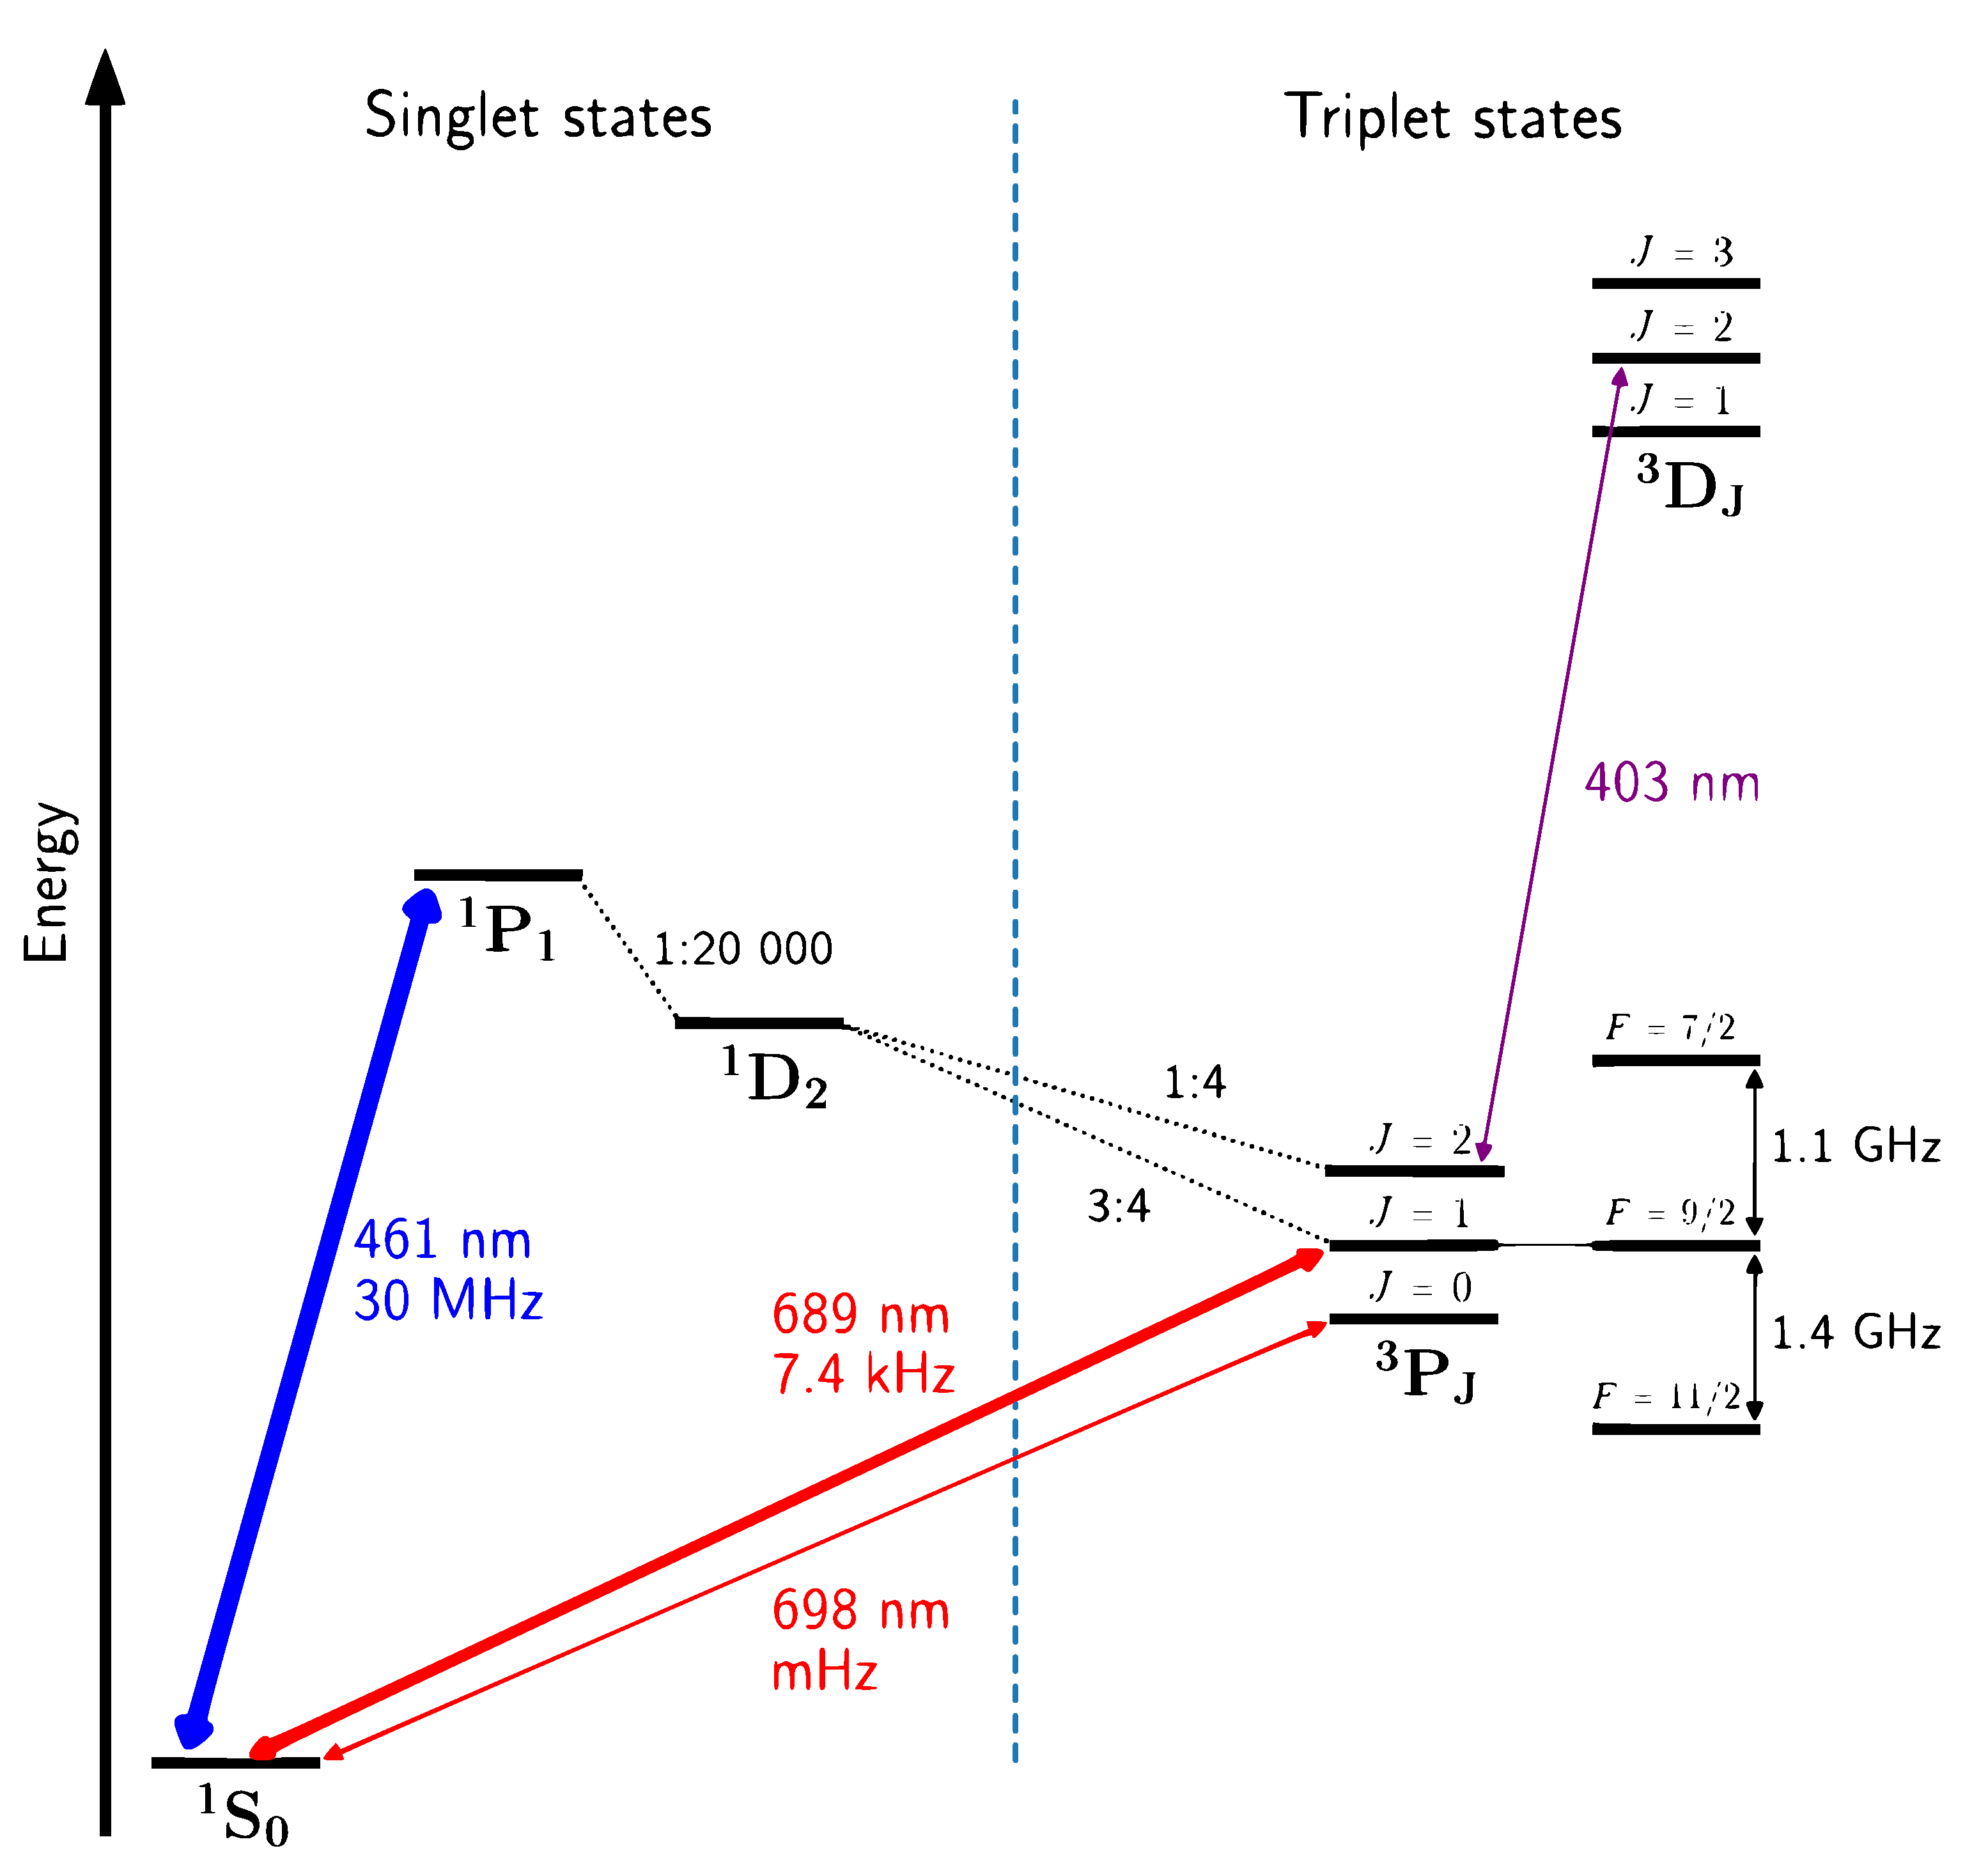
\includegraphics[width=\linewidth, height=0.58\textheight, keepaspectratio]{energy_levels_sr.pdf}
    \end{column}
  \end{columns}
  \amretenir{Un système à grand nombre d'états, robuste et adressable optiquement.}
\end{frame}

\begin{frame}{Pourquoi ? Métrologie et information quantiques}
  \begin{columns}[c]
    \begin{column}{0.5\textwidth}
      \begin{itemize}
        \item<1-> Qudits : plus d'information par atome
        \item<2-> Précision d'un interféromètre à $N$ atomes :
          \begin{itemize}
            \item limite standard : $\Delta\phi = 1/\sqrt{N}$
            \item limite de Heisenberg : $\Delta\phi = 1/N$
          \end{itemize}
        \item<3-> Deux leviers : \alert{contrôle cohérent} à un corps,
          \textcolor{vert}{dissipation} à deux corps
      \end{itemize}
    \end{column}
    \begin{column}{0.45\textwidth}
      \centering
      \figurevide{5.5cm}{4.5cm}
      % schéma : SQL vs Heisenberg, ou vue d'ensemble qudit / paires d'atomes
    \end{column}
  \end{columns}
\end{frame}

\begin{frame}{Ce que j'ai fait en trois ans}
  \begin{enumerate}
    \item<1-> \textbf{Isoler et manipuler des pseudo-spins}\\
      {\small\color{vert} Point fort : au-delà de Stern-Gerlach, isolation de deux états parmi dix}
    \item<2-> \textbf{Mesurer dans des espaces de Hilbert réduits}\\
      {\small\color{vert} Point fort : deux observables non commutables en une seule réalisation}
    \item<3-> \textbf{Dissiper à deux corps par photoassociation}\\
      {\small\color{vert} Point fort : vers la limite de Heisenberg ; inexploré sur $^3P_1$}\\
      {\small\color{violet} Résultat surprenant : nombre et largeur des raies}
  \end{enumerate}
\end{frame}

\begin{frame}{Le dispositif expérimental}
  \begin{columns}[c]
    \begin{column}{0.4\textwidth}
      \begin{itemize}
        \item Refroidissement laser (bleu, puis rouge)
        \item Piège dipolaire croisé, évaporation
        \item Gaz de quelques \si{\micro K}, $\langle n\rangle\sim\SI{e13}{cm^{-3}}$
        \item Détection : imagerie d'absorption
      \end{itemize}
    \end{column}
    \begin{column}{0.56\textwidth}
      \centering
      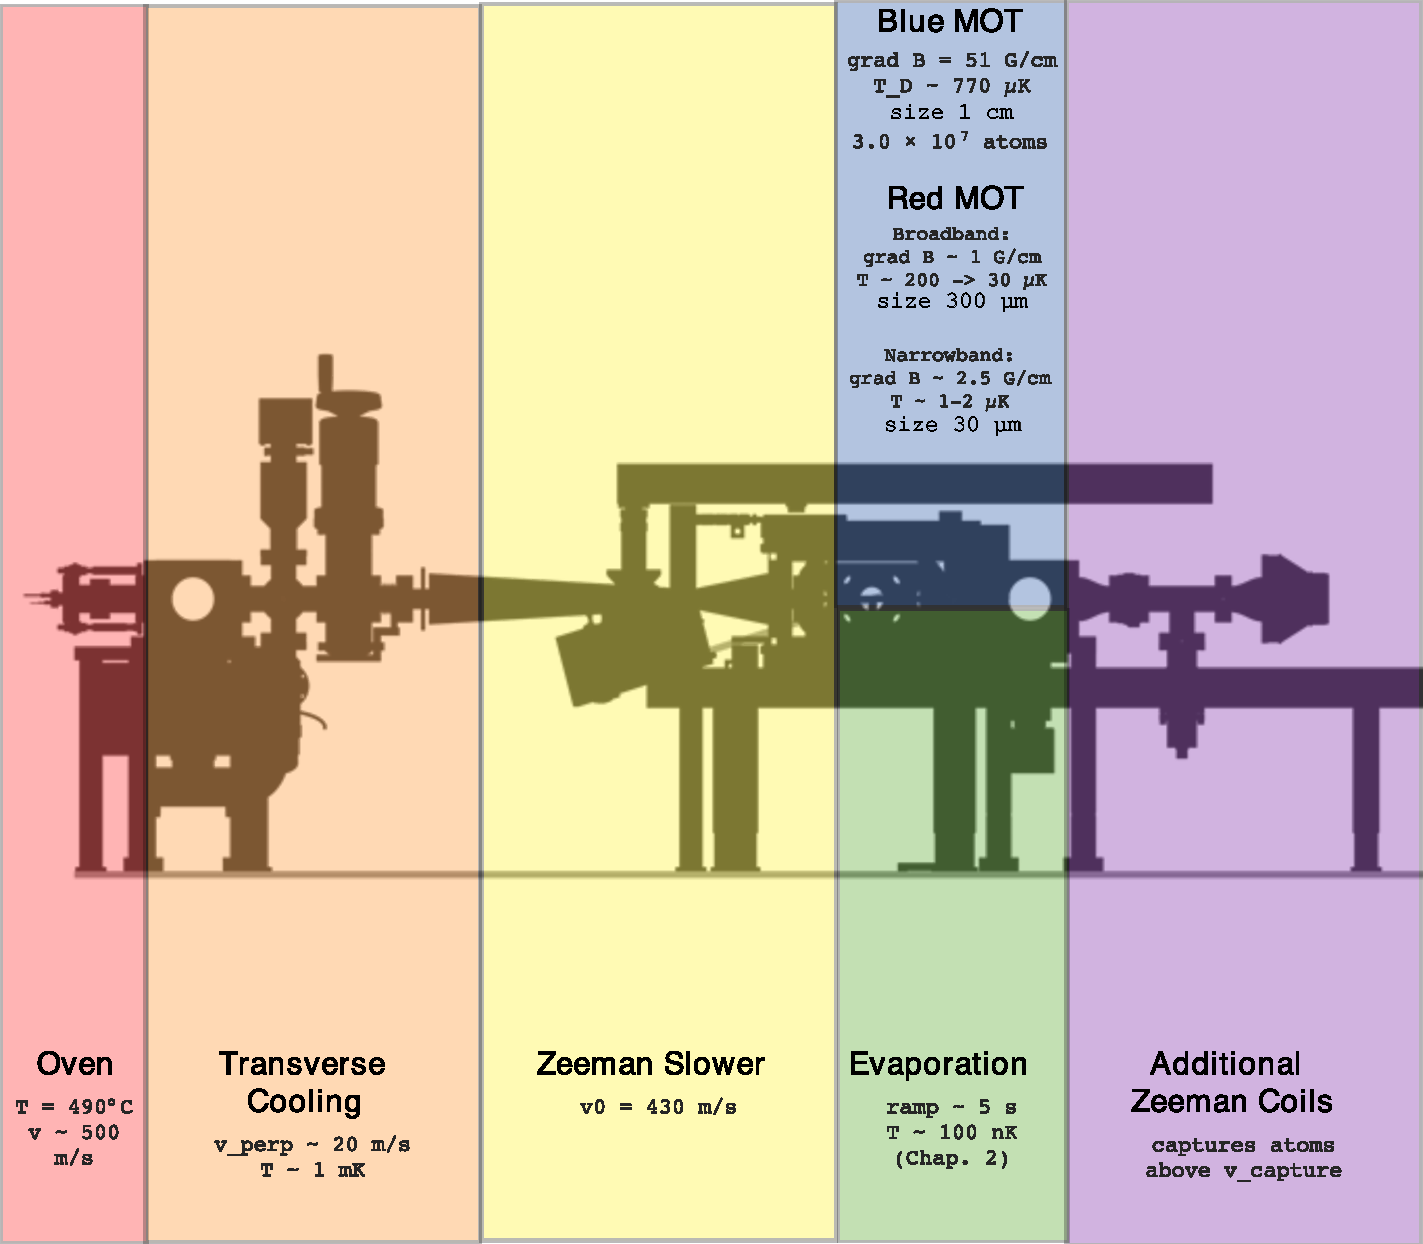
\includegraphics[width=\linewidth, height=0.7\textheight, keepaspectratio]{setup_exp.pdf}
    \end{column}
  \end{columns}
\end{frame}

% =====================================================================
\section{Manipulations cohérentes}  % ~15 min

\begin{frame}{Isoler deux états parmi dix}
  \begin{columns}[c]
    \begin{column}{0.42\textwidth}
      \begin{itemize}
        \item<1-> Faisceau $\pi$ désaccordé dans la structure hyperfine de $^3P_1$
        \item<2-> Déplacement lumineux \alert{tensoriel} : $U(m_F) = q\,m_F^2$
        \item<3-> Les transitions $\delta m_F$ deviennent résolues : une paire d'états = un \alert{pseudo-spin 1/2}
      \end{itemize}
    \end{column}
    \begin{column}{0.54\textwidth}
      \centering
      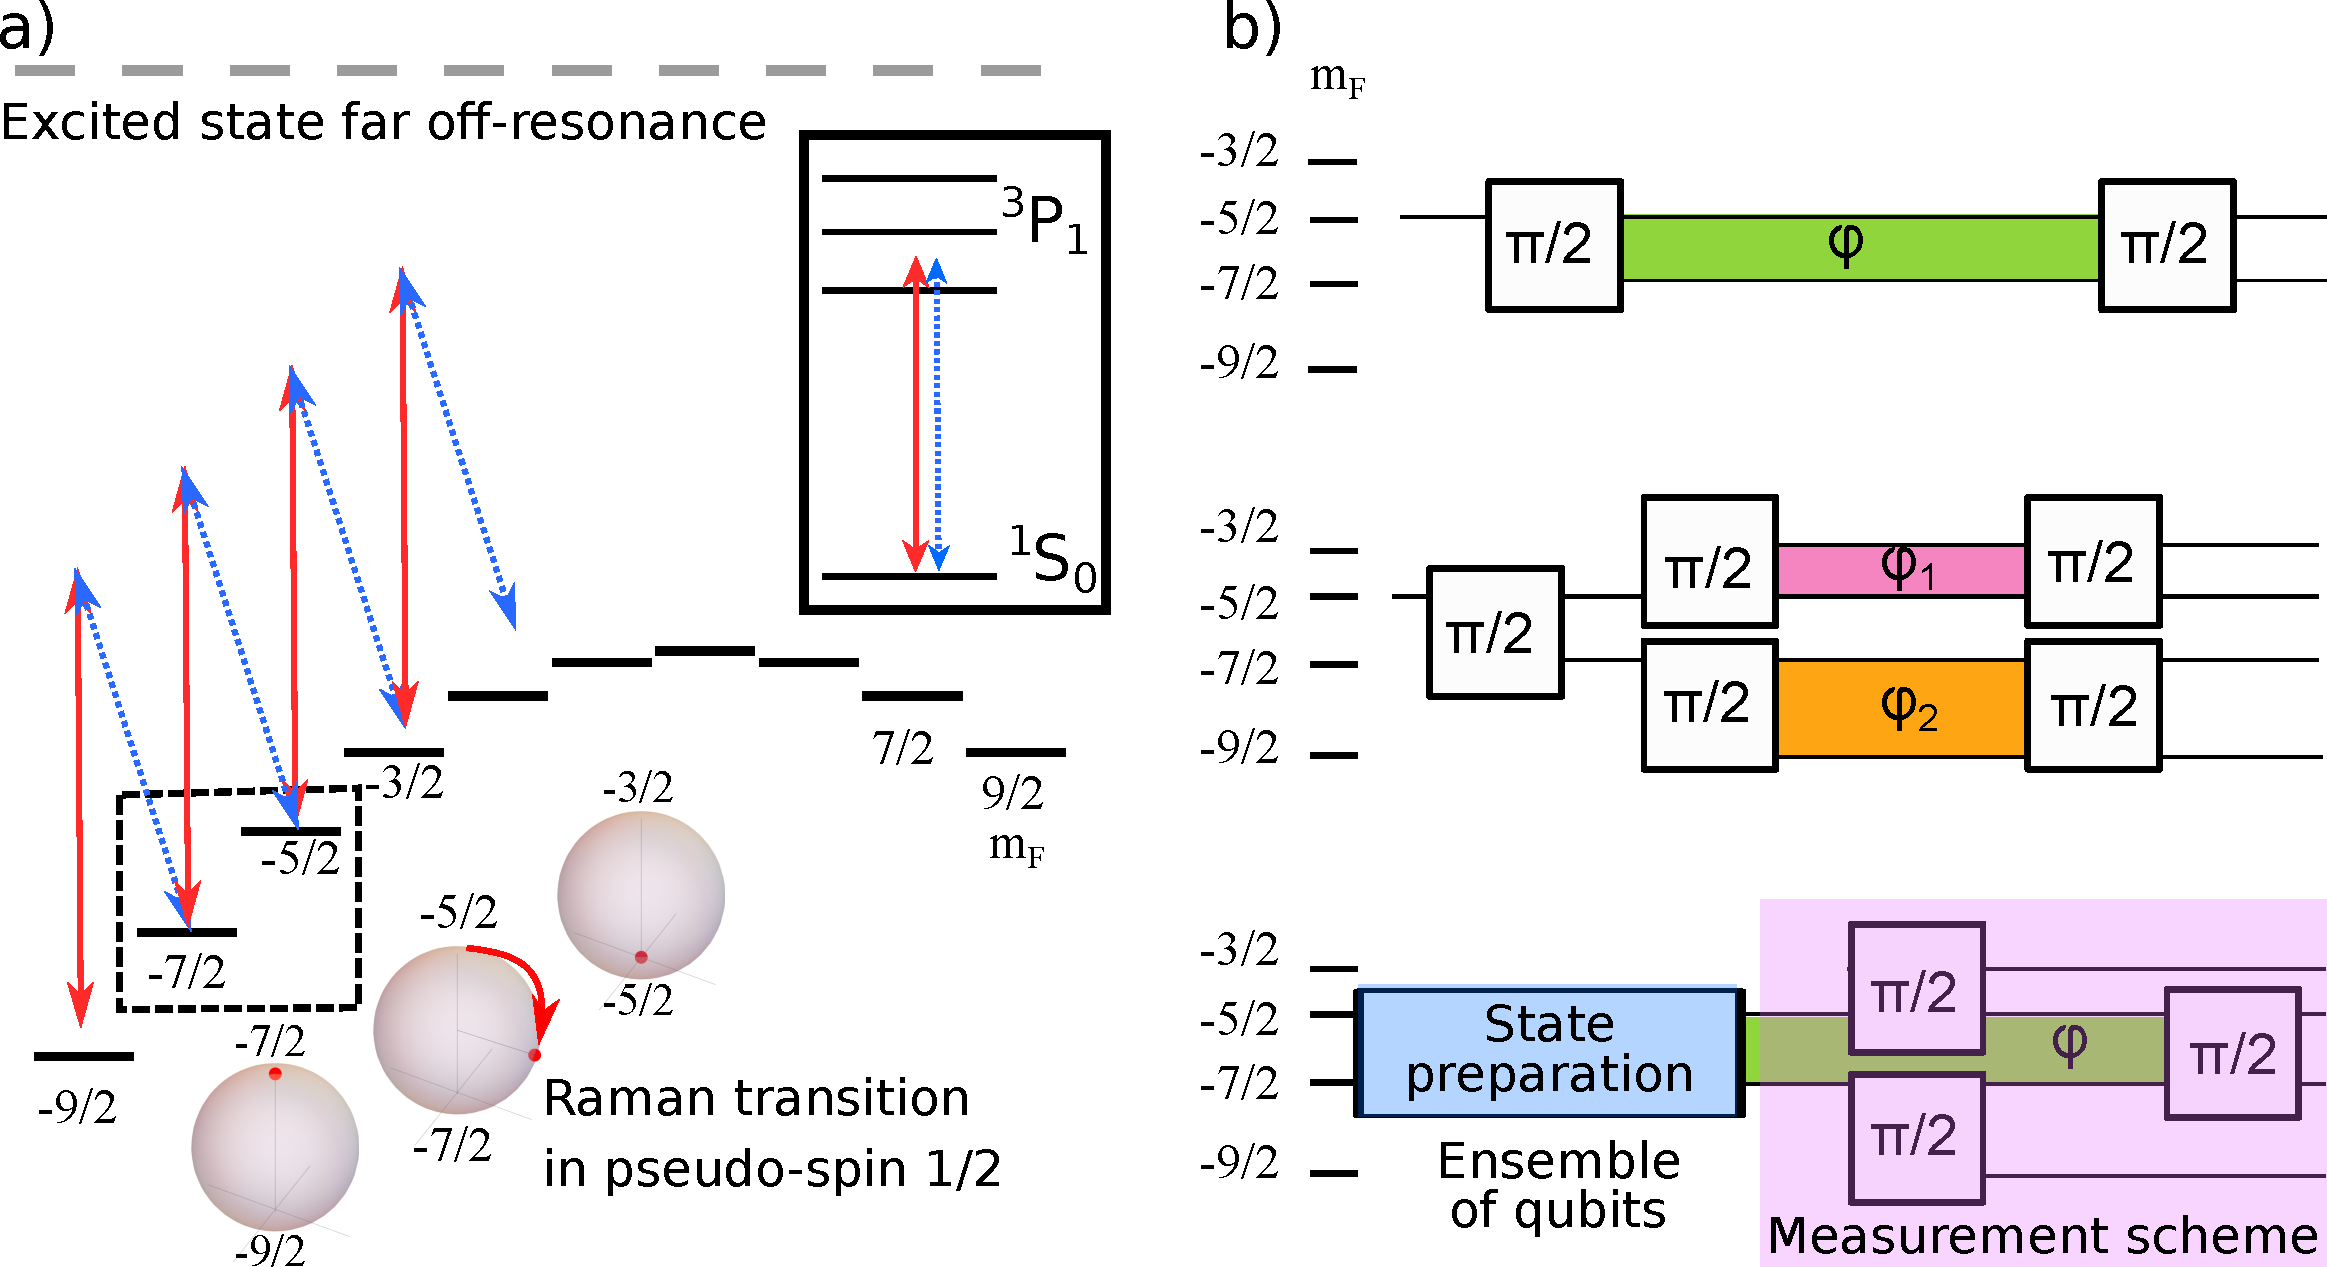
\includegraphics[width=\linewidth, height=0.72\textheight, keepaspectratio]{Fig1.pdf}
    \end{column}
  \end{columns}
\end{frame}

\begin{frame}{Préparer des états cohérents}
  \begin{columns}[c]
    \begin{column}{0.4\textwidth}
      \begin{itemize}
        \item Oscillations de Rabi Raman ($\delta m_F = 1$)
        \item Les états voisins ne sont pas affectés
        \item Amortissement en \SI{298(17)}{ms}
      \end{itemize}
    \end{column}
    \begin{column}{0.56\textwidth}
      \centering
      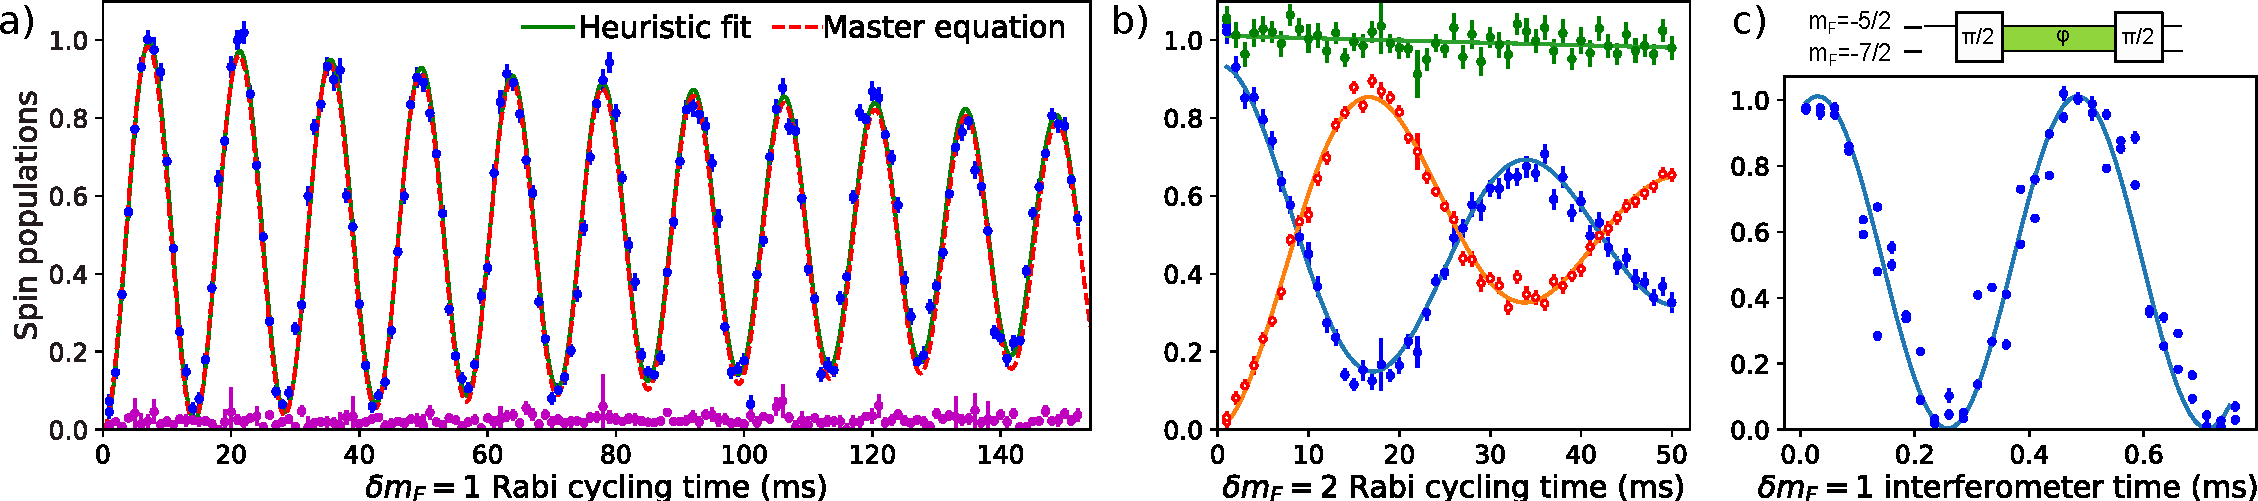
\includegraphics[width=\linewidth, height=0.72\textheight, keepaspectratio]{Fig2.pdf}
    \end{column}
  \end{columns}
\end{frame}

\begin{frame}{Contrôle de phase et cohérence du qubit}
  \begin{columns}[c]
    \begin{column}{0.4\textwidth}
      \begin{itemize}
        \item Interféromètre de Ramsey entre $m_F=-5/2$ et $-7/2$
        \item Analyse de la phase et du contraste
        \item \acompleter{temps de cohérence obtenu}
      \end{itemize}
    \end{column}
    \begin{column}{0.56\textwidth}
      \centering
      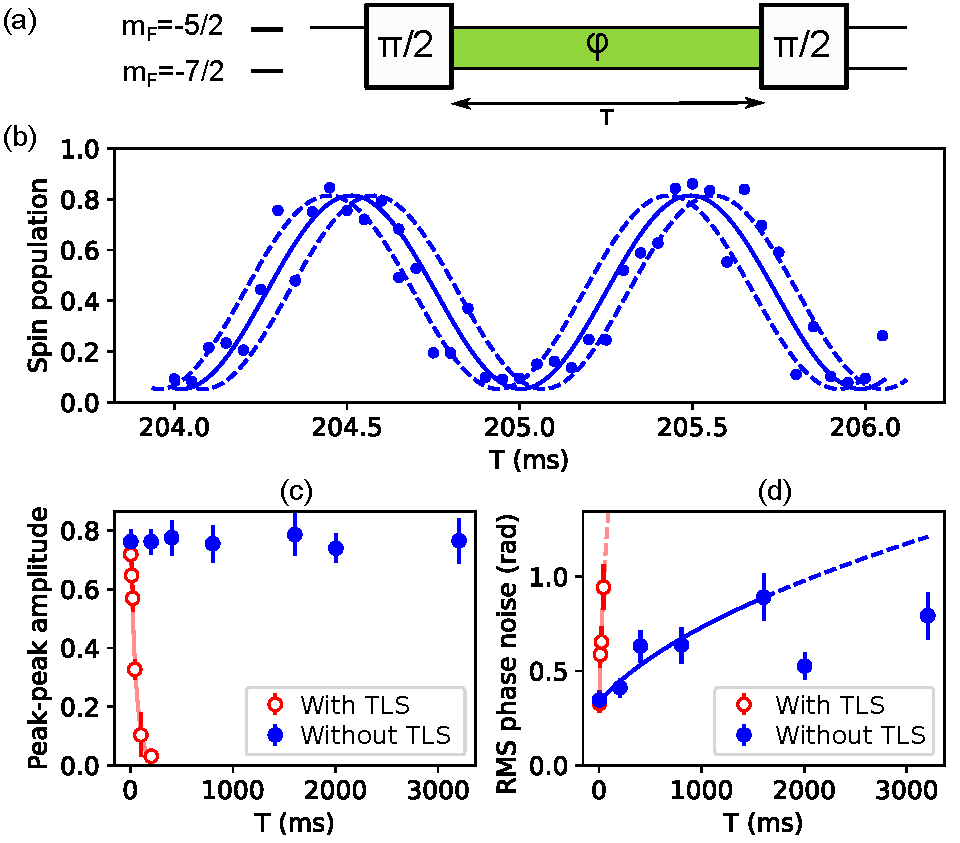
\includegraphics[width=\linewidth, height=0.72\textheight, keepaspectratio]{Fig3.pdf}
    \end{column}
  \end{columns}
\end{frame}

\begin{frame}{Mesurer deux grandeurs physiques à la fois}
  \begin{columns}[c]
    \begin{column}{0.4\textwidth}
      \begin{itemize}
        \item Double interféromètre sur quatre états $m_F$
        \item Deux énergies différentes : deux périodes
        \item Corrélation des deux phases $\phi_1$, $\phi_2$
      \end{itemize}
    \end{column}
    \begin{column}{0.56\textwidth}
      \centering
      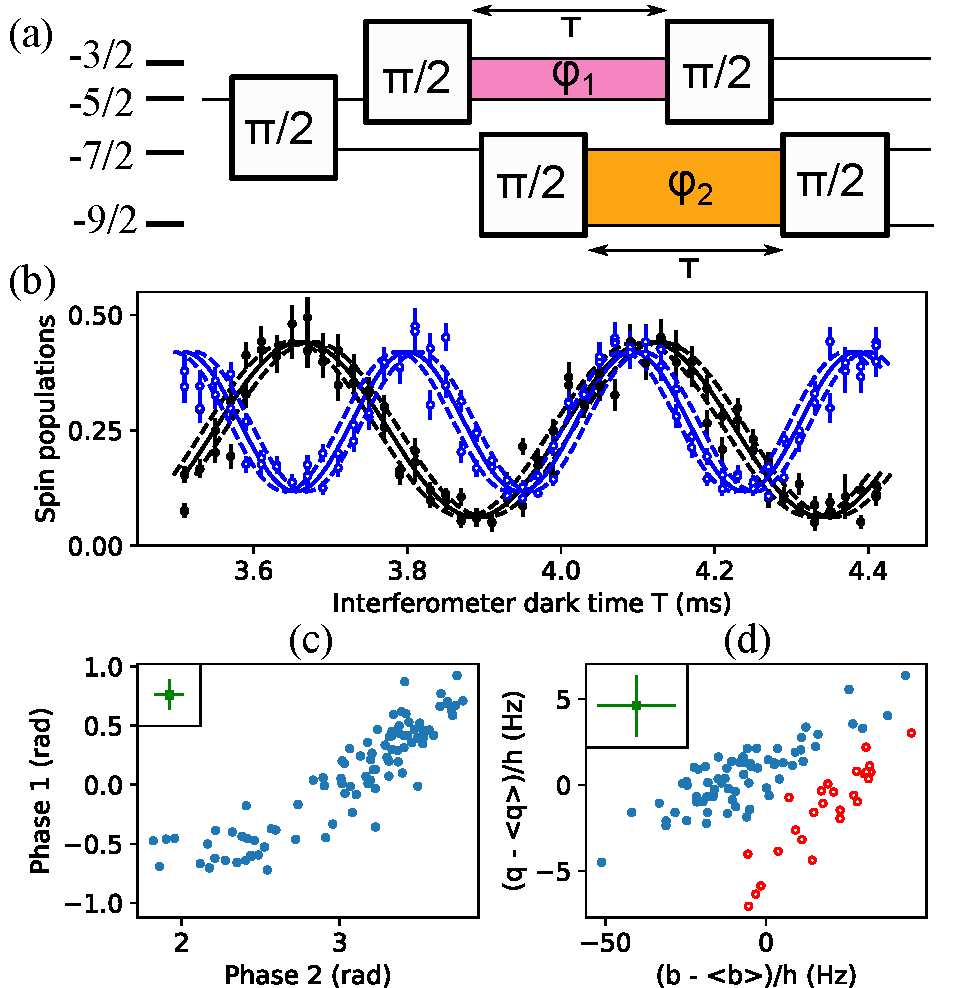
\includegraphics[width=\linewidth, height=0.72\textheight, keepaspectratio]{Fig4.pdf}
    \end{column}
  \end{columns}
\end{frame}

\begin{frame}{Deux observables non commutables en une réalisation}
  \begin{columns}[c]
    \begin{column}{0.4\textwidth}
      \begin{itemize}
        \item Une étape de préparation, une étape de mesure
        \item Opérations unitaires avant la détection des populations
        \item Simulation (équation maîtresse) : un seul paramètre ajusté
      \end{itemize}
    \end{column}
    \begin{column}{0.56\textwidth}
      \centering
      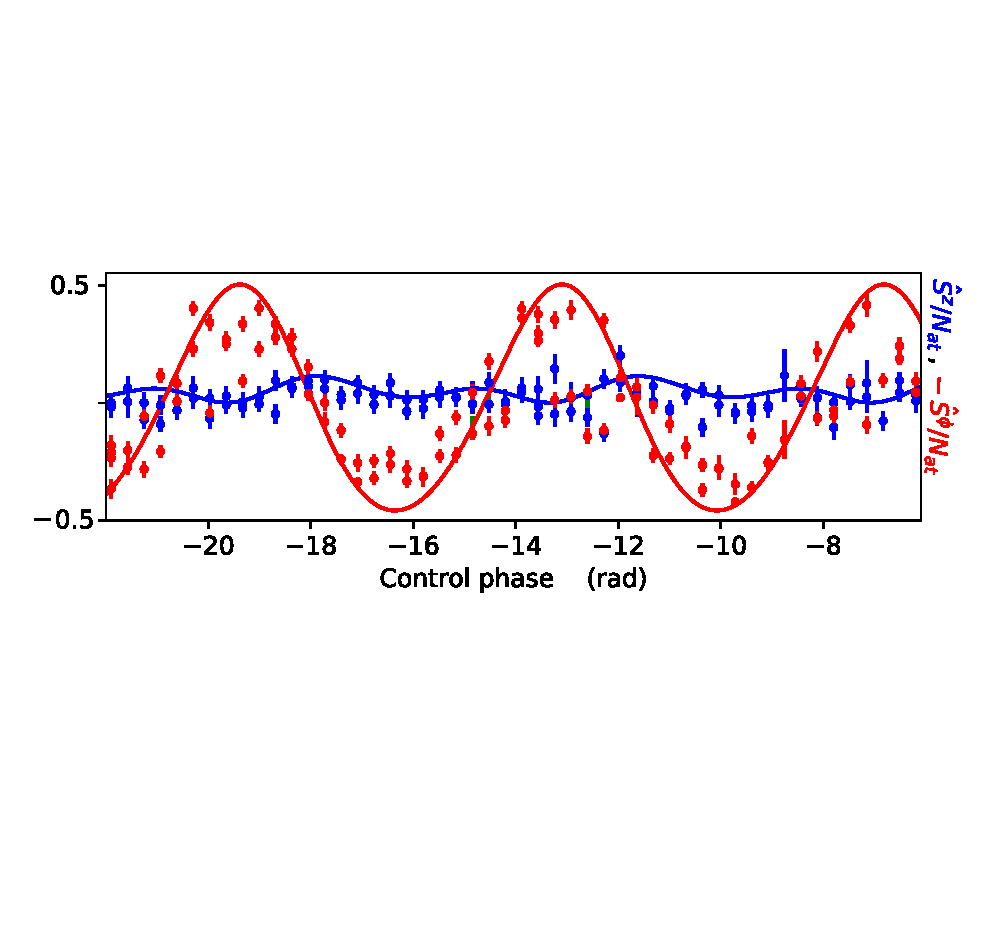
\includegraphics[width=\linewidth, height=0.72\textheight, keepaspectratio,
                       trim=14 166 14 128, clip]{Fig5_v2.pdf}
    \end{column}
  \end{columns}
\end{frame}

\begin{frame}{Limites et extensions}
  \begin{itemize}
    \item<1-> Limites : \acompleter{à compléter}
    \item<2-> Extension à six états : mesurer trois observables
    \item<3-> \acompleter{conséquence sur la variance}
  \end{itemize}
  \amretenir{Un contrôle cohérent de pseudo-spins dans un espace à dix états.}
\end{frame}

% =====================================================================
\section{Photoassociation du \Sr{87}}  % ~20 min

\begin{frame}{La photoassociation}
  \begin{columns}[c]
    \begin{column}{0.48\textwidth}
      \begin{itemize}
        \item<1-> \textbf{Élastique} : énergie cinétique conservée, atomes piégés
        \item<2-> \textbf{Inélastique} : énergie interne libérée, atomes éjectés
        \item<3-> PA : un laser couple une paire à un \alert{état moléculaire excité}
        \item<4-> Désexcitation : atomes chauds ou molécule, donc \alert{perdus}
      \end{itemize}
    \end{column}
    \begin{column}{0.48\textwidth}
      \centering
      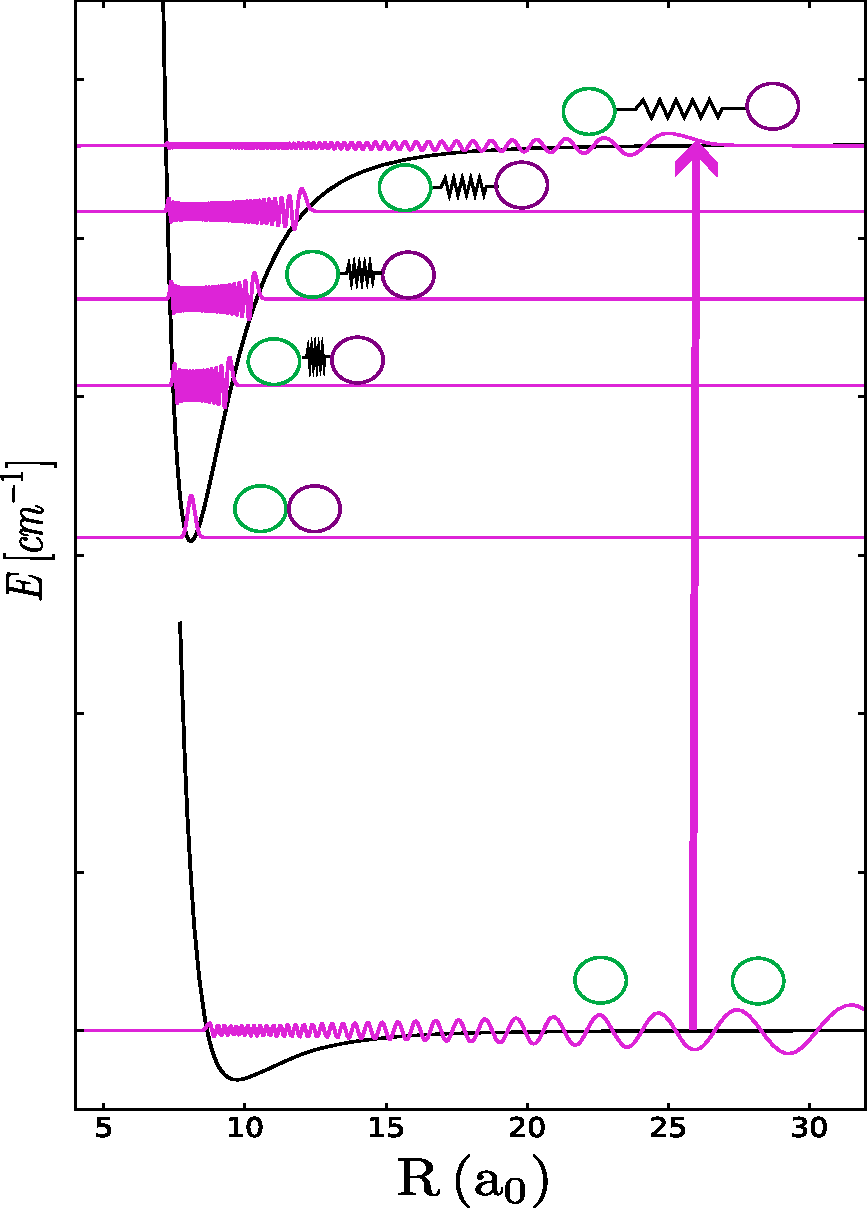
\includegraphics[width=\linewidth, height=0.5\textheight, keepaspectratio]{Figures_pour_theorie/Guttridge_PA_process.pdf}
      \par\source{Adapté de Guttridge \textit{et al.}, 2019}
    \end{column}
  \end{columns}
  \only<4>{\amretenir{Une raie moléculaire = un creux dans le nombre d'atomes.}}
\end{frame}

\begin{frame}{Une perte à deux corps}
  \begin{block}{Dynamique des pertes}
    \centering
    $\dfrac{dN}{dt} = -\beta N^2 - \Gamma N$, \qquad $\beta \propto K_2 / V_e(T)$
  \end{block}
  \begin{itemize}
    \item<2-> $K_2$ : la force de la raie (ne dépend pas de la densité)
    \item<3-> $K_2 \propto l_{\text{opt}}$, et $l_{\text{opt}} \propto I$ : on compare $l_{\text{opt}}/I$
  \end{itemize}
  \only<4->{%
  \begin{alertblock}{Raie élargie}
    \centering
    $K_2(\text{résonance}) = \dfrac{16h}{m_{\text{at}}}\,\dfrac{l_{\text{opt}}}{\eta}$,
    \qquad $\eta = \dfrac{\Gamma_{\text{fit}}}{\Gamma_{\text{rad}}/2\pi}$
  \end{alertblock}}
  \only<5>{\amretenir{Une raie $\eta$ fois trop large a un $K_2$ $\eta$ fois plus faible.}}
\end{frame}

\begin{frame}{Pourquoi la photoassociation du \Sr{87} ?}
  \begin{columns}[c]
    \begin{column}{0.55\textwidth}
      \begin{itemize}
        \item<1-> PA sur $^1S_0$--$^3P_1$ bien connue pour \Sr{88}, \Sr{84}, \Sr{86}
        \item<2-> \Sr{87} : seulement sur $^1P_1$ ; spectre dense sur $^3P_1$ (structure hyperfine)
        \item<3-> Idée (Foss-Feig 2012) : la dissipation à deux corps comme \alert{moteur}
        \item<4-> État stationnaire de Dicke ($m=0$) : vers $\Delta\phi\propto 1/N$
      \end{itemize}
    \end{column}
    \begin{column}{0.4\textwidth}
      \centering
      \figurevide{5cm}{4.5cm}
      % schéma : pertes sélectives en spin -> état de Dicke
    \end{column}
  \end{columns}
  \only<4>{\amretenir{Première étape : identifier les raies moléculaires.}}
\end{frame}

\begin{frame}{Le protocole}
  \begin{columns}[c]
    \begin{column}{0.42\textwidth}
      \begin{itemize}
        \item<1-> Repère : la transition atomique $^1S_0\to{}^3P_1$
        \item<2-> On balaye le laser de PA dans le rouge
        \item<3-> Illumination (\SI{1}{s}), puis on compte les atomes restants
        \item<4-> Raie = creux : ajustement lorentzien (centre, largeur)
      \end{itemize}
    \end{column}
    \begin{column}{0.54\textwidth}
      \centering
      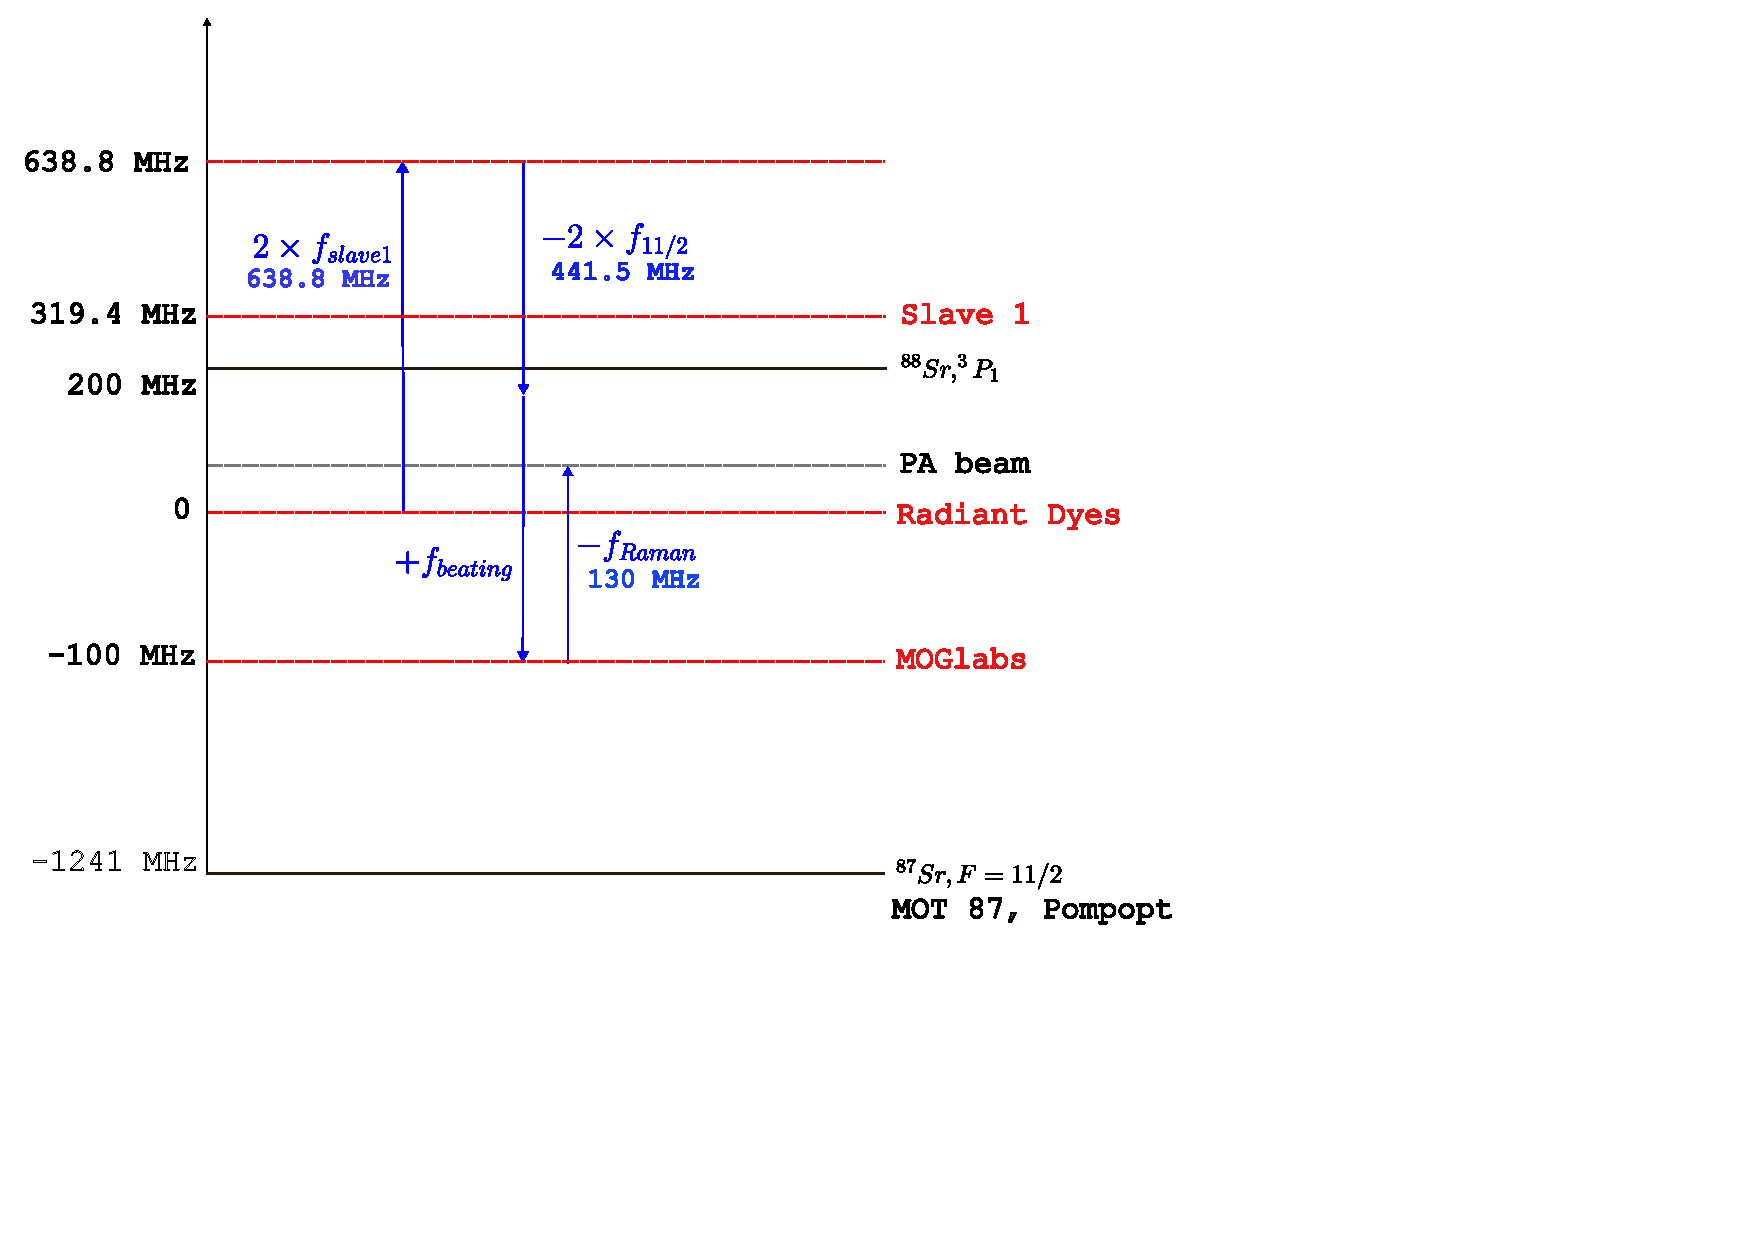
\includegraphics[width=\linewidth, height=0.7\textheight, keepaspectratio]{frequences_PA_88.pdf}
    \end{column}
  \end{columns}
\end{frame}

\begin{frame}{Validation sur le \Sr{88} : les spectres}
  \begin{columns}[c]
    \begin{column}{0.4\textwidth}
      \begin{itemize}
        \item $\nu=-1$ et $\nu=-2$ retrouvées
        \item Positions à moins de \SI{0.5}{MHz} de la littérature
        \item Largeur $\approx\SI{330}{kHz}$ ($\eta\approx22$)
      \end{itemize}
    \end{column}
    \begin{column}{0.56\textwidth}
      \centering
      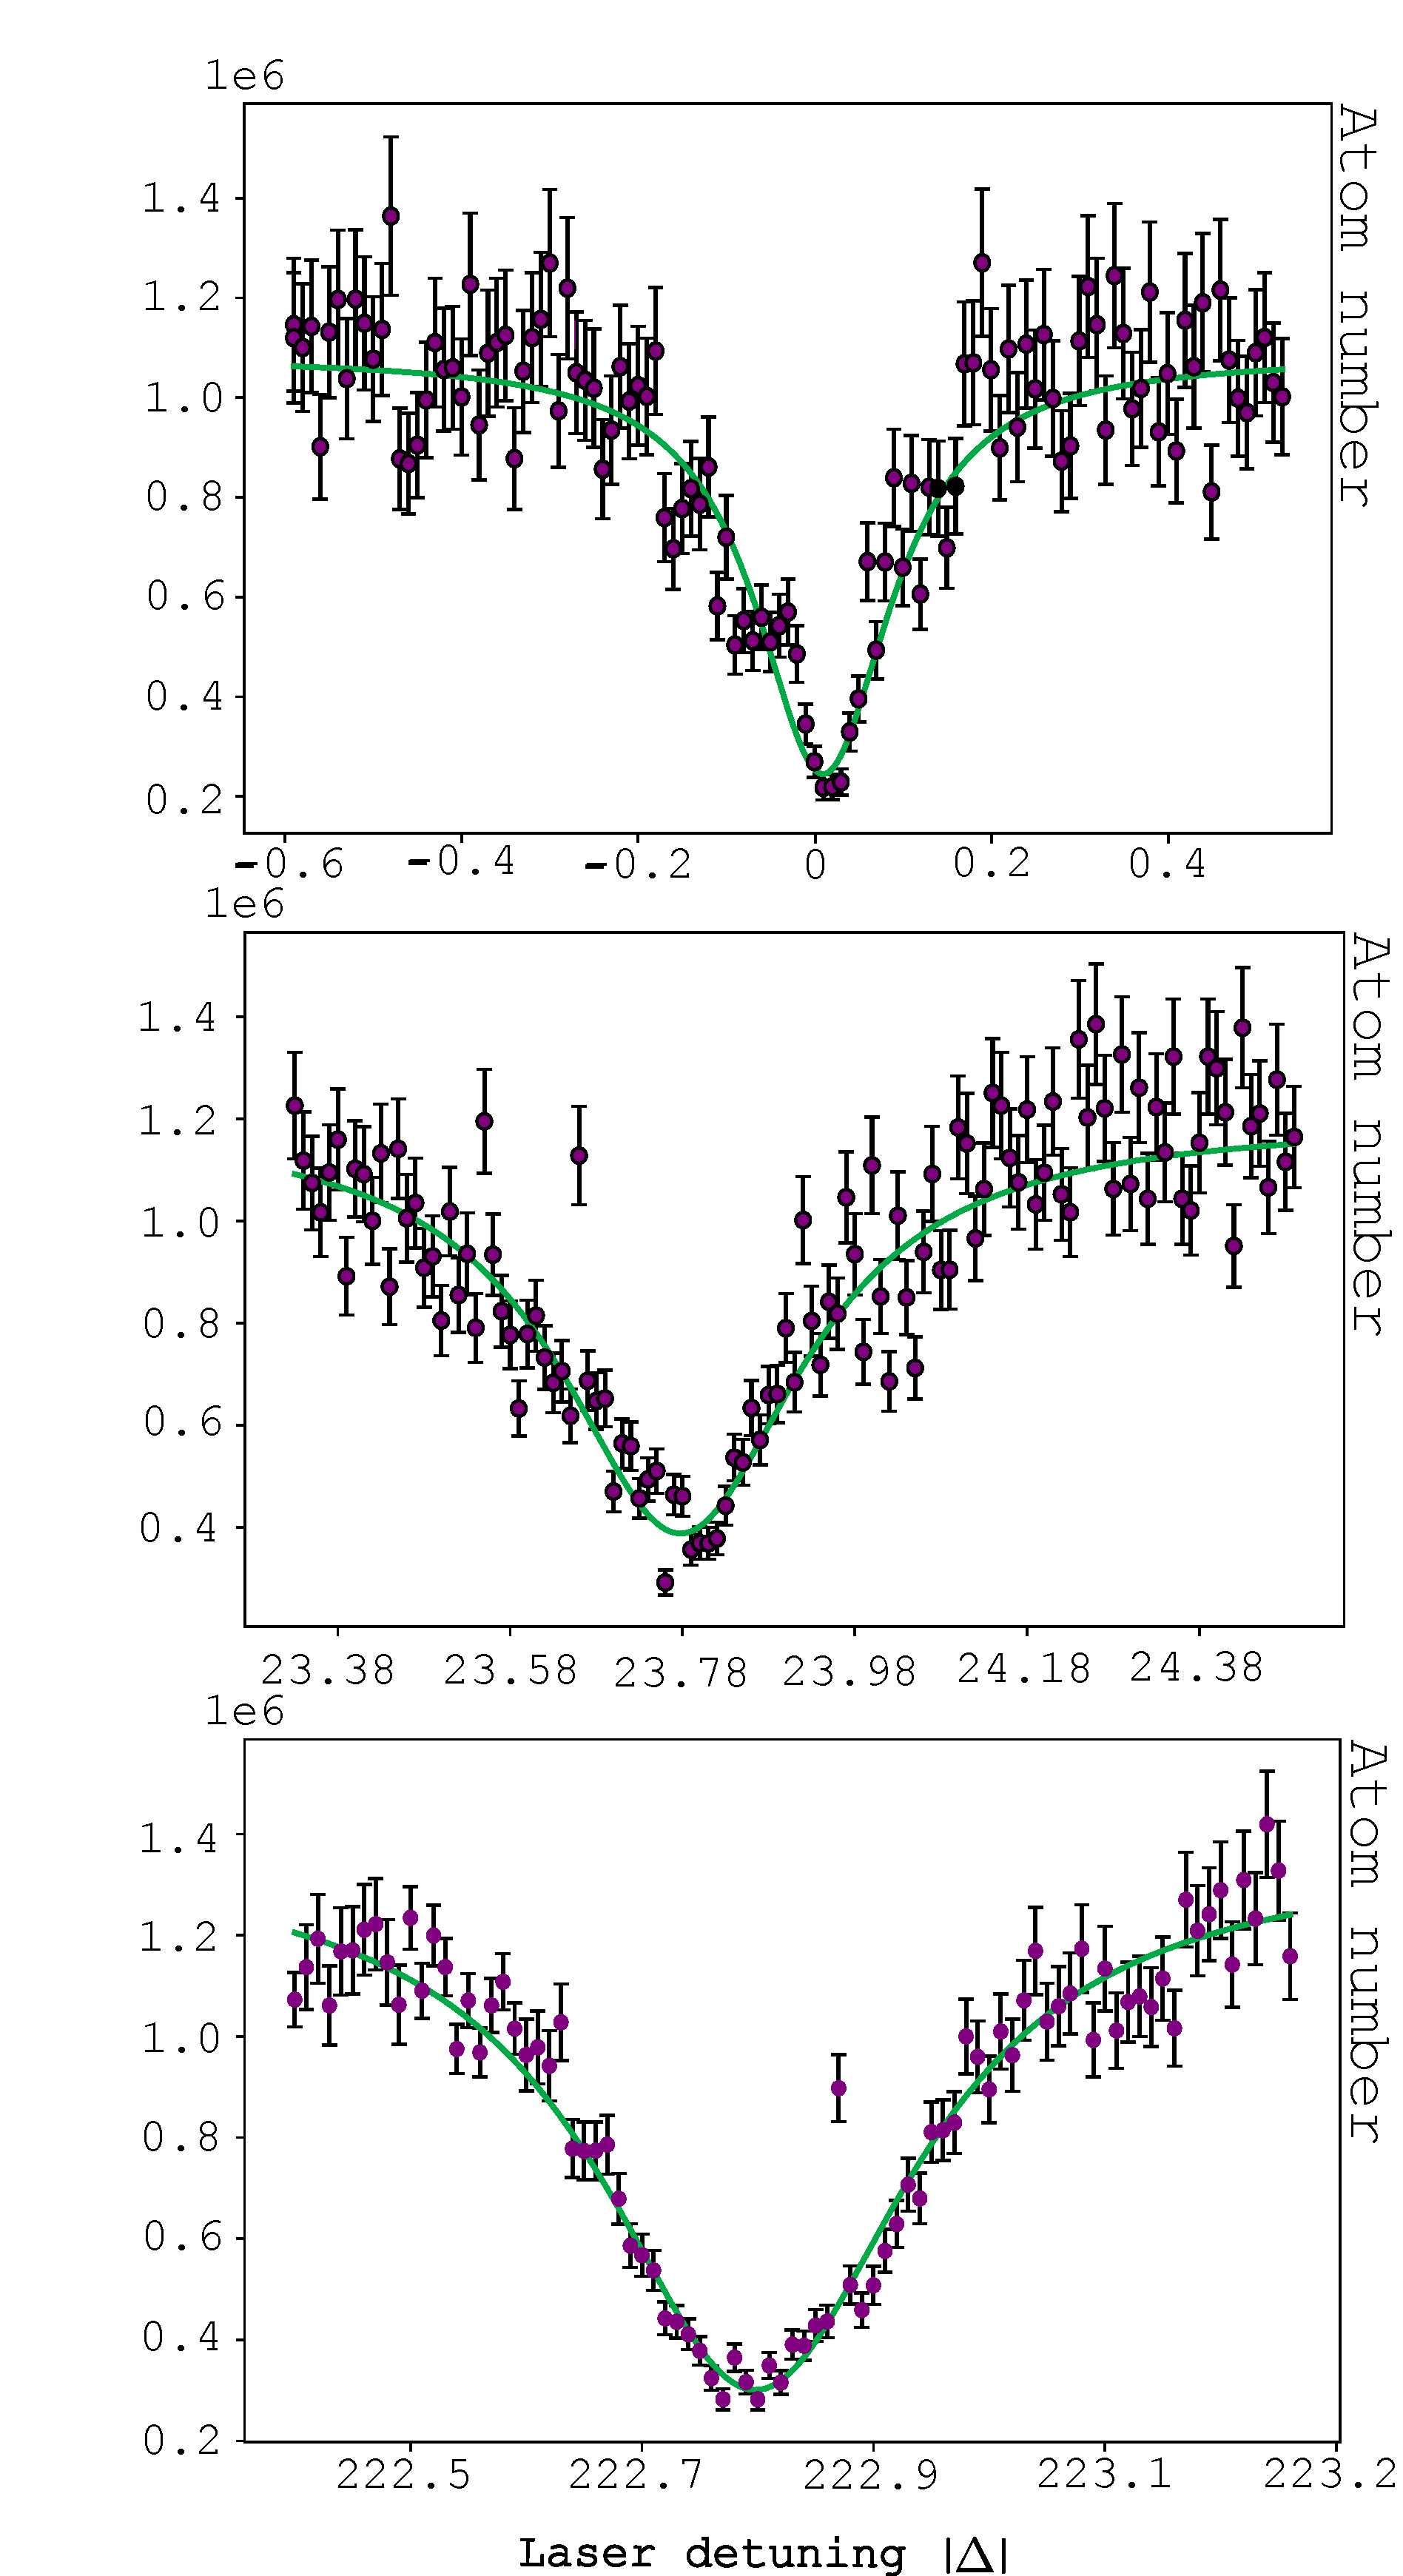
\includegraphics[width=\linewidth, height=0.74\textheight, keepaspectratio]{88Sr/resonance_88.pdf}
    \end{column}
  \end{columns}
\end{frame}

\begin{frame}{Validation sur le \Sr{88} : le déclin $N(t)$}
  \begin{columns}[c]
    \begin{column}{0.4\textwidth}
      \begin{itemize}
        \item<1-> Temps courts : deux corps (non exponentiel)
        \item<2-> Temps longs : un corps (droite en échelle log)
        \item<3-> Ajustement : $K_2$, puis $l_{\text{opt}}/I$
        \item<4-> $\nu=-2$ : $56\pm10$ contre $68(3)$ $a_0$/(W/cm$^2$) (Blatt 2011)
      \end{itemize}
    \end{column}
    \begin{column}{0.56\textwidth}
      \centering
      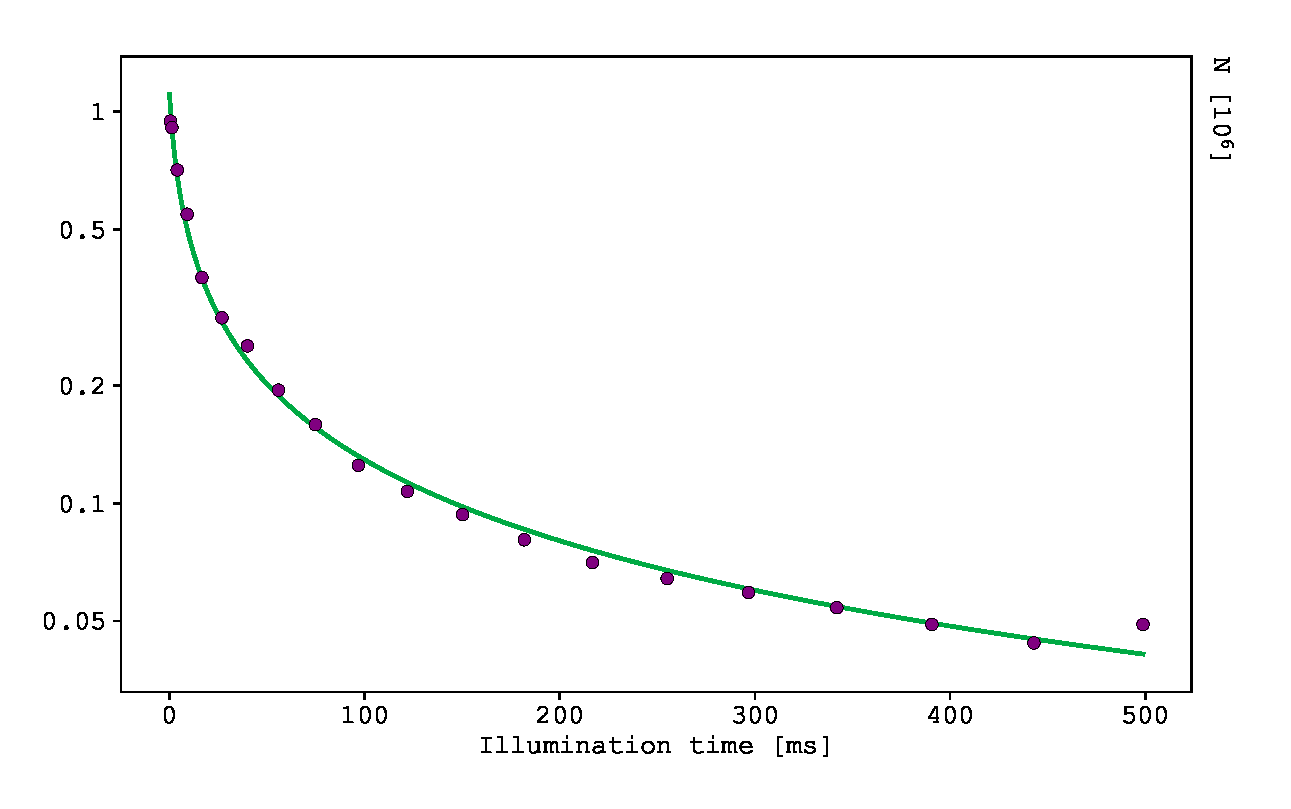
\includegraphics[width=0.85\linewidth, height=0.3\textheight, keepaspectratio]{88Sr/fig_149_sr88.pdf}\\
      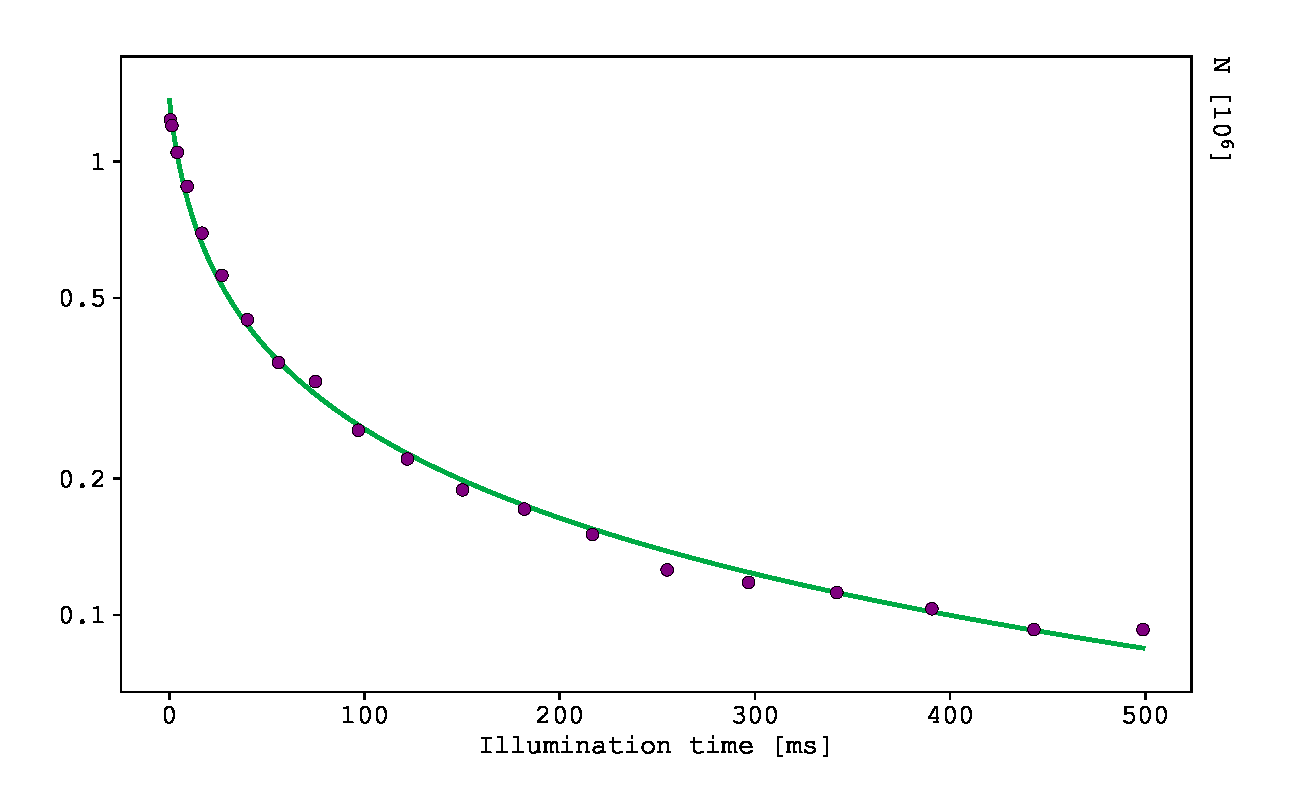
\includegraphics[width=0.85\linewidth, height=0.3\textheight, keepaspectratio]{88Sr/fig_148_sr88.pdf}
    \end{column}
  \end{columns}
  \only<4>{\amretenir{Montage validé : accord avec la littérature à un facteur $\lesssim 2$.}}
\end{frame}

\begin{frame}{Reconnaître une vraie raie moléculaire}{Une leçon tirée d'un faux signal}
  \begin{columns}[c]
    \begin{column}{0.44\textwidth}
      \begin{itemize}
        \item<1-> À \SI{-6}{MHz} : déclin non exponentiel\ldots
        \item<2-> \ldots{} mais signal \alert{atomique} : bande latérale de bruit du laser
        \item<3-> La forme de $N(t)$ seule ne suffit pas
        \item<4-> Test : chercher la même perte à $+\delta$ et $-\delta$ de l'atome
      \end{itemize}
    \end{column}
    \begin{column}{0.52\textwidth}
      \centering
      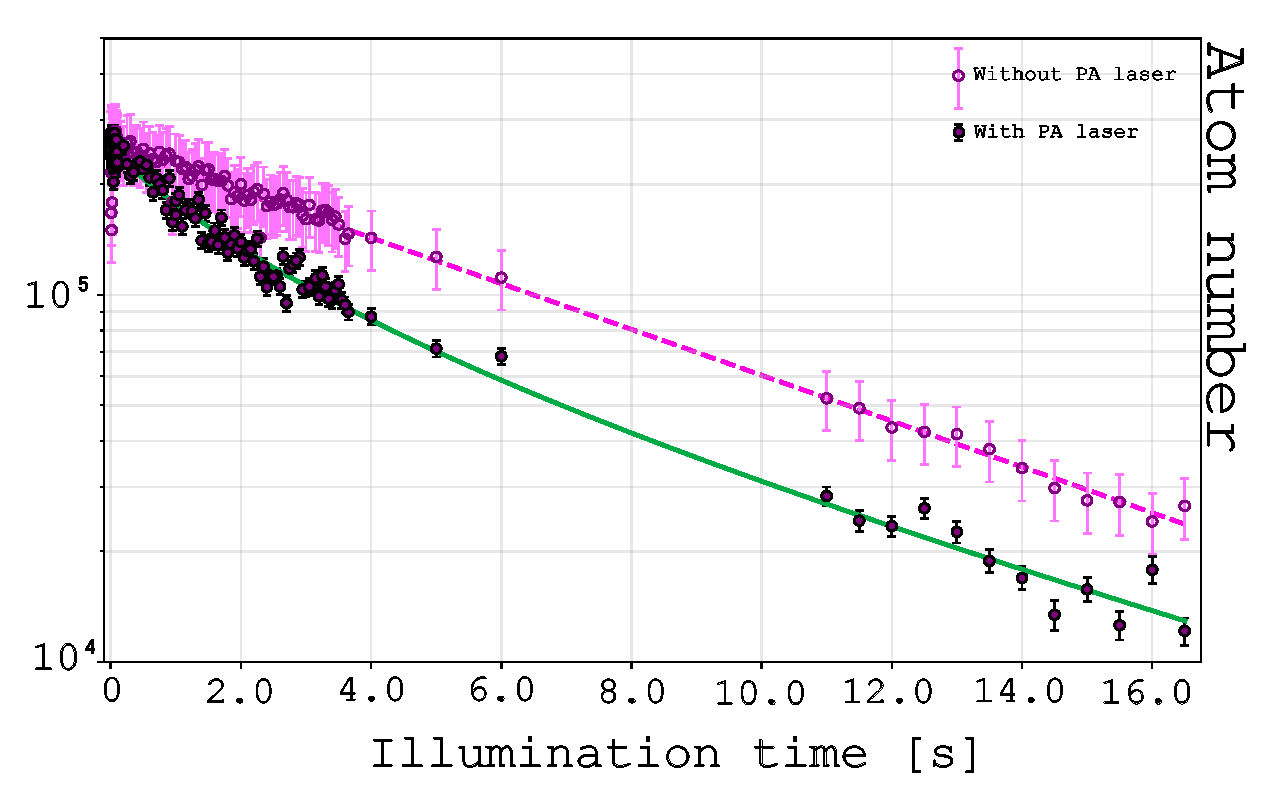
\includegraphics[width=\linewidth, height=0.7\textheight, keepaspectratio]{87Sr/data16_exp_bruit_6MHz.pdf}
    \end{column}
  \end{columns}
\end{frame}

\begin{frame}{Ce que l'on attend pour le \Sr{87}}
  \begin{columns}[c]
    \begin{column}{0.44\textwidth}
      \begin{itemize}
        \item<1-> Largeur : $\Gamma_{\text{rad}}/2\pi\approx\SI{15}{kHz}$
        \item<2-> $\sim 3\times10^3$ raies dans les \SI{380}{MHz} explorés
        \item<3-> Positions prédites par loi d'échelle en masse
      \end{itemize}
    \end{column}
    \begin{column}{0.52\textwidth}
      \centering
      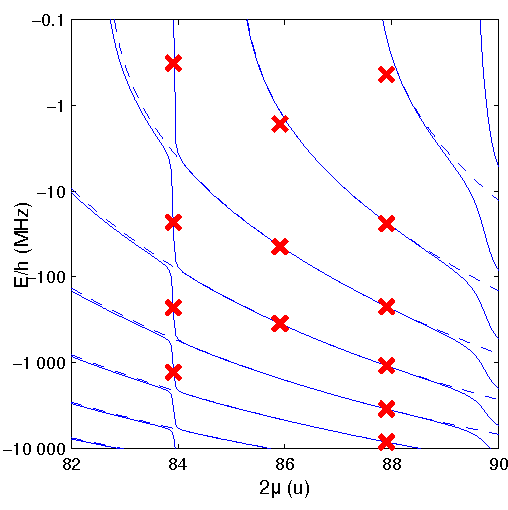
\includegraphics[width=\linewidth, height=0.68\textheight, keepaspectratio]{Figures_pour_theorie/mass_scaling.pdf}
      \par\source{Borkowski \textit{et al.}, 2014}
    \end{column}
  \end{columns}
\end{frame}

\begin{frame}{Ce que l'on observe : une raie en détail}
  \centering
  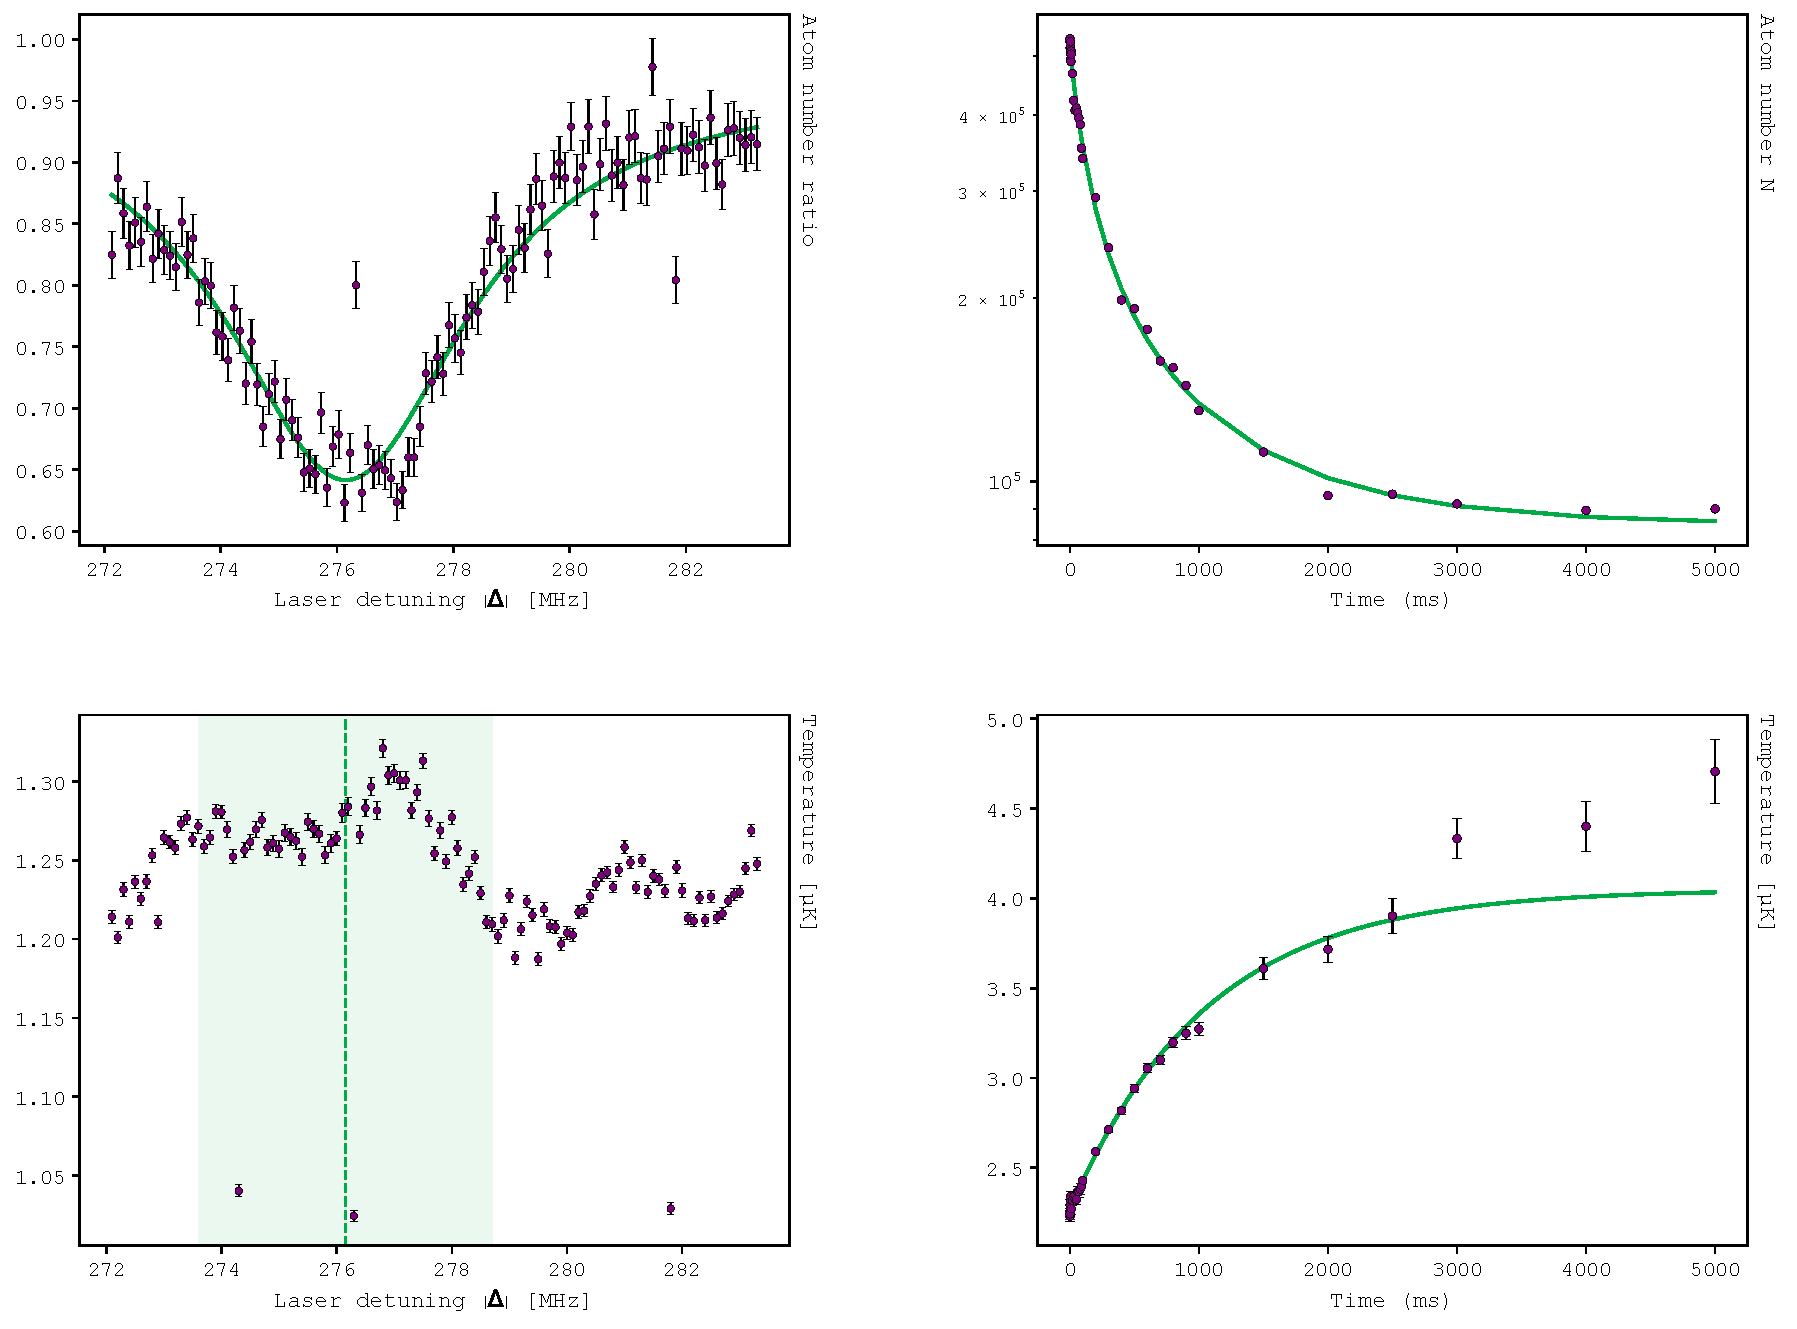
\includegraphics[width=\linewidth, height=0.64\textheight, keepaspectratio]{87Sr/composite_276MHz.pdf}
  \par\source{Raie à \SI{-276.83}{MHz} \textperiodcentered{}
    spectre : $I=\SI{5.2}{W/cm^2}$, $\langle n\rangle=\SI{1.6e13}{cm^{-3}}$ \textperiodcentered{}
    déclin : $I=\SI{31}{W/cm^2}$, $\langle n\rangle=\SI{7.8e12}{cm^{-3}}$ \textperiodcentered{}
    illumination \SI{1}{s}}
\end{frame}

\begin{frame}{Seulement trois raies}
  \centering
  \begin{tabular}{@{}lccc@{}}
    \toprule
    Raie (MHz) & $-259.01$ & $-276.83$ & $-377.2$ \\
    \midrule
    Largeur $\Gamma_{\text{fit}}$ (MHz) & $7.4\pm0.9$ & $5.0\pm0.3$ & $20.2\pm2.3$ \\
    Profondeur après \SI{1}{s} & $40\%$ & $35\%$ & $9\%$ \\
    Temps caractéristique $\tau$ & \SI{286}{ms} & \SI{117}{ms} & \SI{5.3}{s} \\
    $l_{\text{opt}}/I$ ($a_0$/(W/cm$^2$)) & $3.4\pm1.9$ & $3.1\pm0.5$ & $0.49\pm0.35$ \\
    \bottomrule
  \end{tabular}
  \par\vspace{0.4cm}
  \begin{itemize}
    \item<2-> Aucune raie à moins de \SI{259}{MHz} de l'asymptote
    \item<3-> Largeurs de 5 à \SI{20}{MHz} au lieu de \SI{15}{kHz}
  \end{itemize}
\end{frame}

\begin{frame}{Où se placent ces raies ?}
  \begin{columns}[c]
    \begin{column}{0.36\textwidth}
      \begin{itemize}
        \item<1-> \textcolor{vert}{\Sr{88}} : sur la littérature
        \item<2-> \textcolor{violet}{\Sr{87}} : 1 à 2 ordres de grandeur plus bas
        \item<3-> Au niveau de la raie la plus faible connue du \Sr{84}
      \end{itemize}
    \end{column}
    \begin{column}{0.6\textwidth}
      \centering
      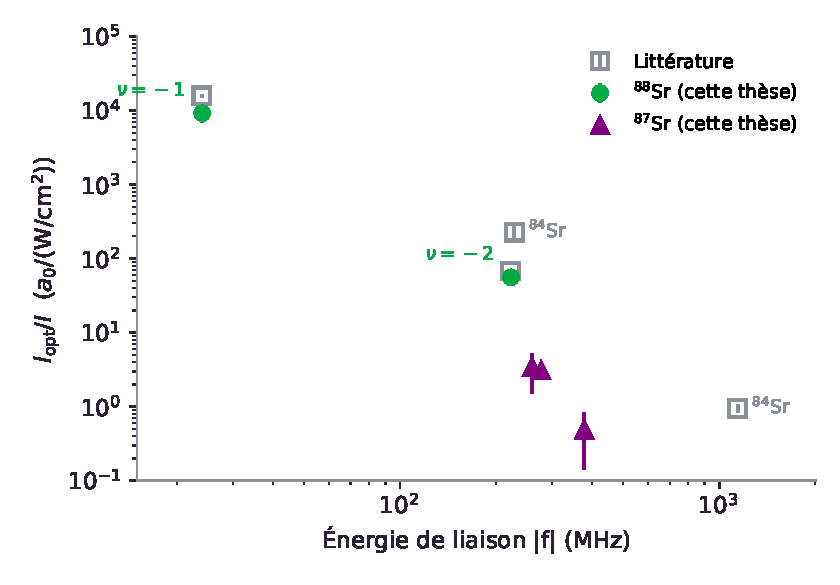
\includegraphics[width=\linewidth, height=0.74\textheight, keepaspectratio]{lopt_comparaison.pdf}
    \end{column}
  \end{columns}
\end{frame}

\begin{frame}{Le vrai message : la largeur}
  \begin{columns}[c]
    \begin{column}{0.36\textwidth}
      \begin{itemize}
        \item<1-> $\eta$ : $1.5 \to 22 \to 330$--$1350$
        \item<2-> $K_2(\text{résonance}) \propto l_{\text{opt}}/\eta$
        \item<3-> Raies peu profondes et raies larges : \alert{le même effet}
      \end{itemize}
    \end{column}
    \begin{column}{0.6\textwidth}
      \centering
      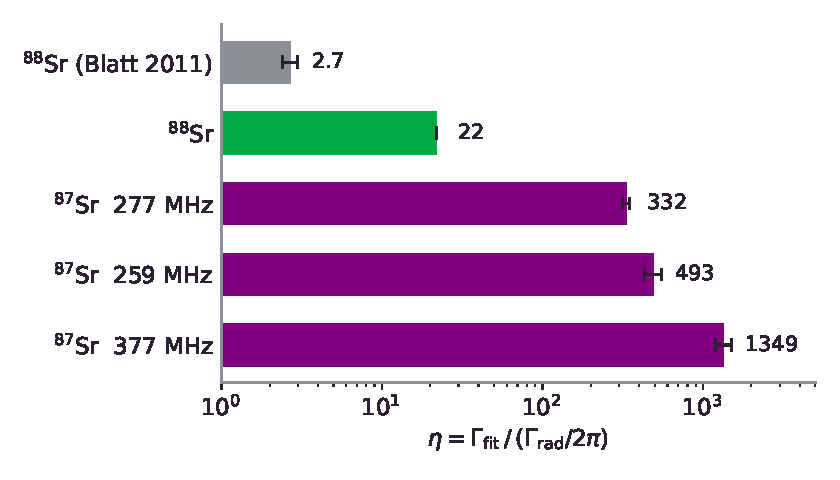
\includegraphics[width=\linewidth, height=0.66\textheight, keepaspectratio]{elargissement_eta.pdf}
    \end{column}
  \end{columns}
\end{frame}

\begin{frame}[standout]
  L'anomalie des raies du \Sr{87} est leur largeur\\[0.3cm]
  {\normalsize\color{white!60} et non leur force}
\end{frame}

\begin{frame}{D'où vient cette largeur ?}
  \begin{columns}[t]
    \begin{column}{0.48\textwidth}
      {\fontforte\color{violet} Causes techniques}\par\vspace{0.2cm}
      \begin{itemize}
        \item Pureté spectrale du laser de PA
        \item Déplacement lumineux inhomogène du faisceau de PA
        \item Lumière du piège : transitions multi-photons, déplacement lumineux
      \end{itemize}
    \end{column}
    \begin{column}{0.48\textwidth}
      {\fontforte\color{vert} Causes physiques}\par\vspace{0.2cm}
      \begin{itemize}
        \item \textbf{Prédissociation} vers $^3P_0$ : raie large, perte faible au pic
        \item Croisements avec des potentiels plus hauts ($^1S_0+{}^1D_2$)
        \item Statistique quantique et sélection de spin : abaissent $l_{\text{opt}}$, mais n'élargissent pas
      \end{itemize}
    \end{column}
  \end{columns}
  \amretenir{Hypothèses les plus probables : prédissociation et déplacements lumineux.}
\end{frame}

\begin{frame}{Les pistes à explorer}
  \begin{columns}[c]
    \begin{column}{0.5\textwidth}
      \small
      {\fontforte\color{gris} Déjà testé, sans effet}\par\vspace{0.1cm}
      \begin{itemize}
        \item Polarisation du laser de PA
        \item Champ magnétique
      \end{itemize}
      \vspace{0.2cm}
      {\fontforte\color{violet} À faire}\par\vspace{0.1cm}
      \begin{itemize}
        \item Largeur en fonction de $I$ : déplacement lumineux ou prédissociation ?
        \item Séquence de \textit{chopping} piège / PA sur le \Sr{87}
        \item Pompage optique : moins de potentiels, moins de prédissociation
      \end{itemize}
    \end{column}
    \begin{column}{0.45\textwidth}
      \centering
      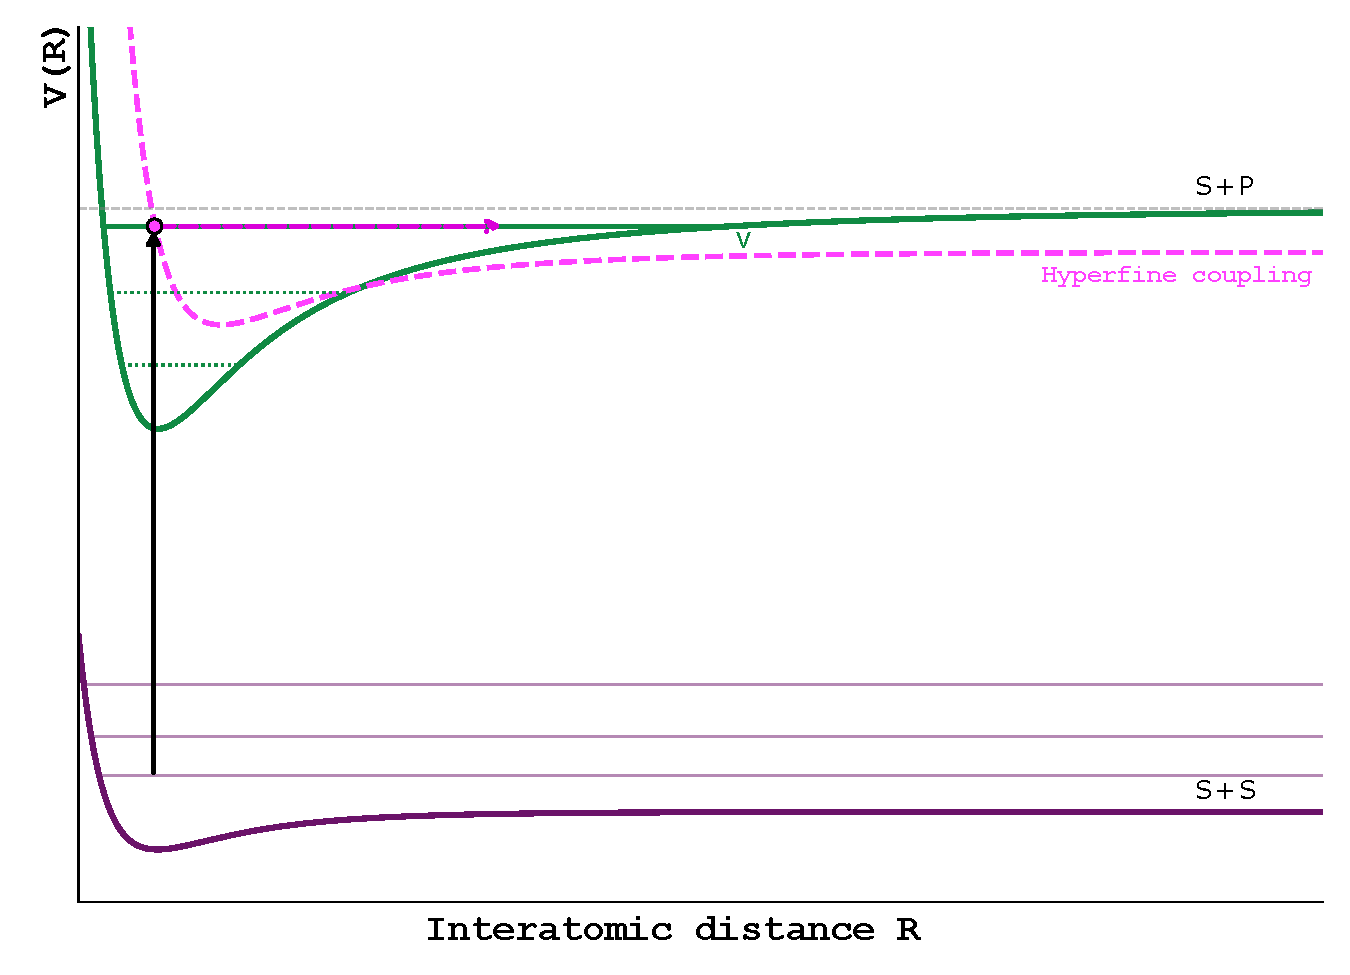
\includegraphics[width=\linewidth, height=0.6\textheight, keepaspectratio]{Figures_pour_theorie/predissociation.pdf}
    \end{column}
  \end{columns}
\end{frame}

% =====================================================================
\section{Conclusion}

\begin{frame}{Conclusion}
  \begin{columns}[t]
    \begin{column}{0.48\textwidth}
      {\fontforte\color{violet} Manipulations cohérentes}\par\vspace{0.2cm}
      \begin{itemize}
        \item Pseudo-spins isolés parmi dix états
        \item Mesure simultanée de deux grandeurs
        \item Deux observables non commutables en une réalisation
      \end{itemize}
    \end{column}
    \begin{column}{0.48\textwidth}
      {\fontforte\color{vert} Photoassociation}\par\vspace{0.2cm}
      \begin{itemize}
        \item Protocole validé sur le \Sr{88}
        \item Trois raies du \Sr{87} sur $^3P_1$
        \item Raies $10^2$ à $10^3$ fois trop larges : une découverte inattendue
      \end{itemize}
    \end{column}
  \end{columns}
  \amretenir{Perspectives : \acompleter{ouverture pour chaque sujet}}
\end{frame}

\begin{frame}[standout]
  Merci de votre attention\\[0.4cm]
  \traitlaser[3cm]
\end{frame}

% ---------------------------------------------------------------------
% Diapos de secours (après \appendix, non comptées dans le total)
\appendix

\begin{frame}{Ajustement de $N(t)$ avec chauffage}
  \begin{block}{Fonction d'ajustement (éq. 3.79 de la thèse)}
    \centering
    $N(t) = \dfrac{N_0 e^{-\Gamma t}}{1 + \left[\dfrac{K_2}{8\pi^{3/2}}\,m_{\text{at}}^{3/2}\,\omega_x\omega_y\omega_z\right] N_0 \displaystyle\int_0^t \left(\frac{1}{k_B T(t')}\right)^{3/2} e^{-\Gamma t'}\,dt'}$
  \end{block}
  \begin{itemize}
    \item $T(t)$ mesurée, interpolée linéairement, \alert{fixée} avant l'ajustement
    \item Paramètres libres : $\Gamma$, $K_2$, $N_0$, offset (minimisation du $\chi^2$)
    \item $K_2$ constant ; $\beta(t)$ varie seulement parce que $T(t)$ varie
  \end{itemize}
\end{frame}

\begin{frame}{Résultats complets sur le \Sr{87}}
  \centering\scriptsize
  \begin{tabular}{@{}lccc@{}}
    \toprule
    Raie (MHz) & $-259.01 \pm 0.12$ & $-276.83 \pm 0.03$ & $-377.2 \pm 0.5$ \\
    \midrule
    \multicolumn{4}{@{}l}{\textit{Spectre}} \\
    Profondeur & $0.40 \pm 0.02$ & $0.35 \pm 0.01$ & $0.09 \pm 0.01$ \\
    Largeur $\Gamma_{\text{fit}}$ (MHz) & $7.4 \pm 0.9$ & $5.0 \pm 0.3$ & $20.2 \pm 2.3$ \\
    $T$ (\si{\micro K}) & $2.38\pm0.08$ & $1.25\pm0.03$ & $2.38\pm0.04$ \\
    $\langle n\rangle$ (\SI{e12}{cm^{-3}}) & $7.0\pm1.0$ & $16\pm2$ & $7.2\pm1.0$ \\
    $I$ (W/cm$^2$) & $19.0\pm1.1$ & $5.2\pm0.3$ & $5.6\pm0.4$ \\
    \midrule
    \multicolumn{4}{@{}l}{\textit{Déclin $N(t)$}} \\
    $I$ (W/cm$^2$) & $19.0\pm1.1$ & $31.0\pm1.8$ & $19.0\pm1.1$ \\
    $\langle n\rangle$ (\SI{e12}{cm^{-3}}) & $7.0\pm1.0$ & $7.8\pm1.1$ & $7.0\pm1.0$ \\
    $K_2$ (\SI{e-13}{cm^3/s}) & $5.0\pm2.8$ & $11\pm2$ & $0.27\pm0.19$ \\
    \midrule
    $\eta$ & $493\pm60$ & $332\pm17$ & $1349\pm155$ \\
    $l_{\text{opt}}/I$, méthode 1 (spectre) & $0.63\pm0.13$ & $0.54\pm0.08$ & $0.84\pm0.17$ \\
    $l_{\text{opt}}/I$, méthode 2 (déclin) & $3.4\pm1.9$ & $3.1\pm0.5$ & $0.49\pm0.35$ \\
    \bottomrule
  \end{tabular}
\end{frame}

\begin{frame}{Les autres raies du \Sr{87}}
  \centering
  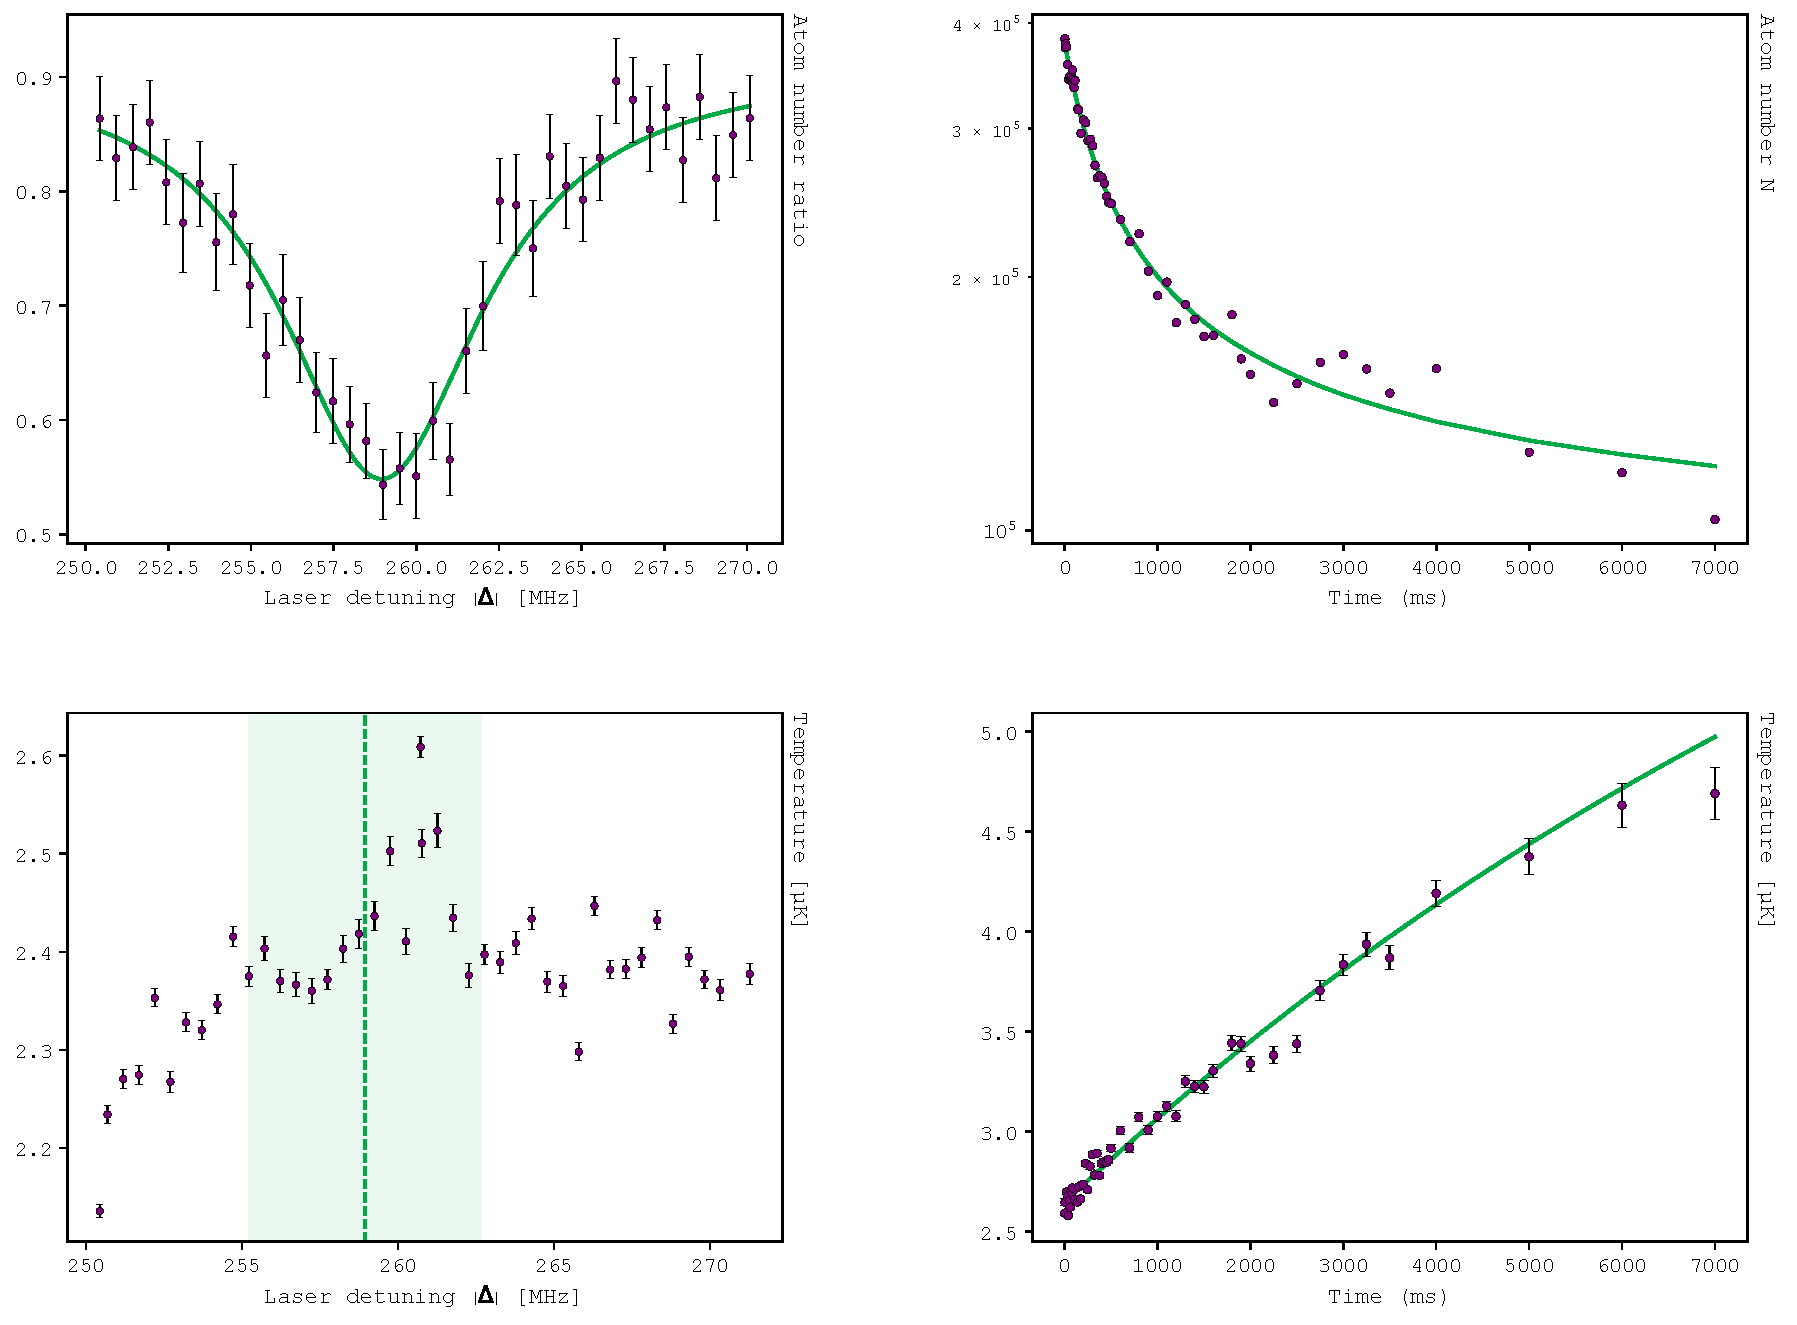
\includegraphics[width=0.49\linewidth, height=0.72\textheight, keepaspectratio]{87Sr/composite_259MHz.pdf}\hfill
  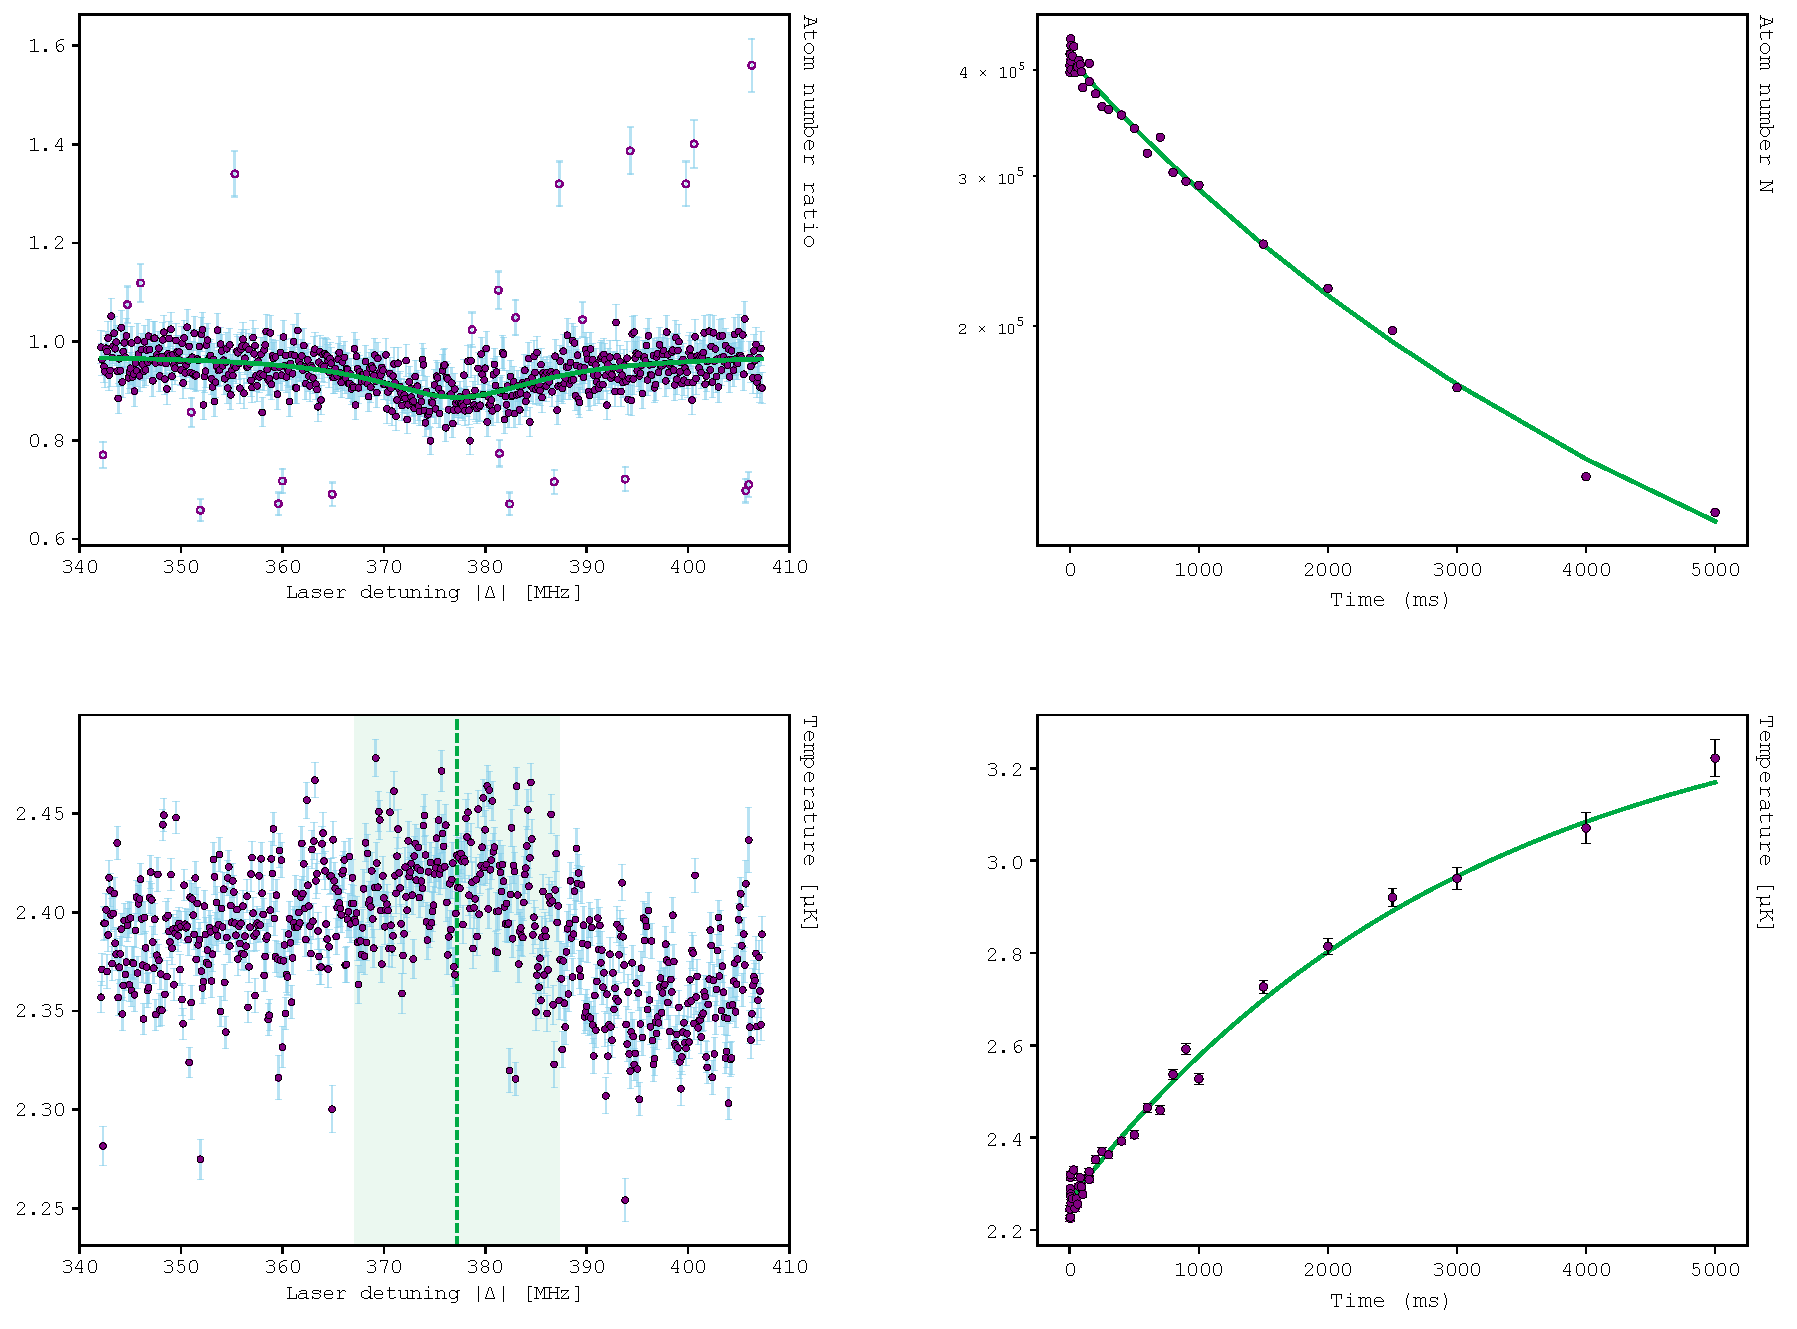
\includegraphics[width=0.49\linewidth, height=0.72\textheight, keepaspectratio]{87Sr/composite_375MHz.pdf}
\end{frame}

\begin{frame}{Effet du laser sur la largeur (\Sr{88})}
  \centering
  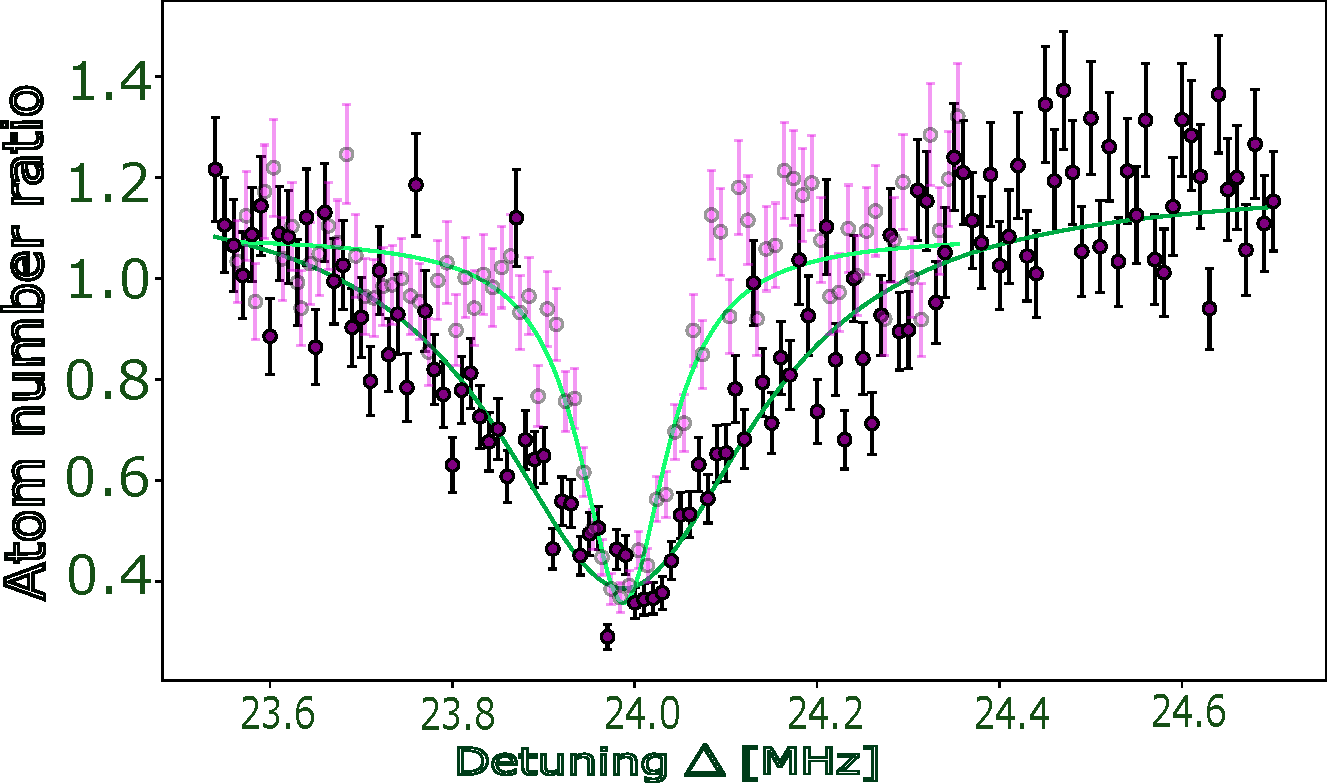
\includegraphics[width=\linewidth, height=0.66\textheight, keepaspectratio]{88Sr/comparaison_raie_24MHz_88_jolie.pdf}
  \par\source{MOGlabs : \SI{231}{kHz} \textperiodcentered{} laser injecté : \SI{122}{kHz}}
\end{frame}

\begin{frame}{Séquence de \textit{chopping} piège / PA}
  \centering
  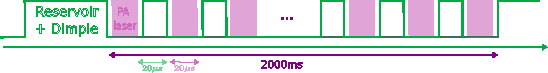
\includegraphics[width=\linewidth, height=0.7\textheight, keepaspectratio]{Figures_pour_theorie/sequence_chopping.pdf}
\end{frame}

\begin{frame}{Le faux signal à $\pm\SI{6}{MHz}$}
  \centering
  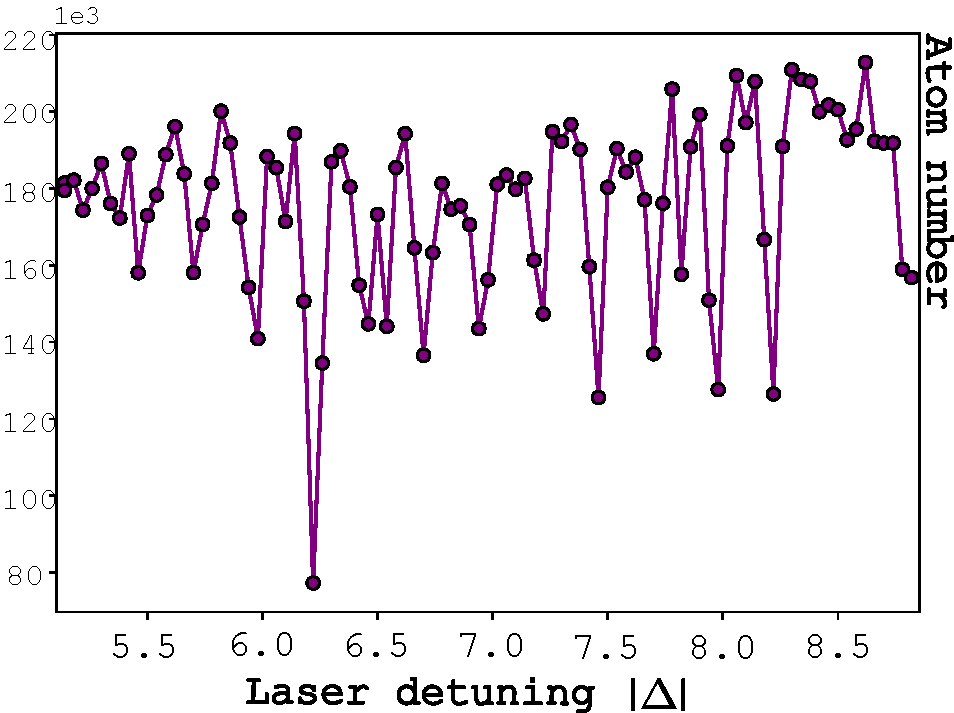
\includegraphics[width=0.49\linewidth, height=0.66\textheight, keepaspectratio]{87Sr/data15_6MHz_noise.pdf}\hfill
  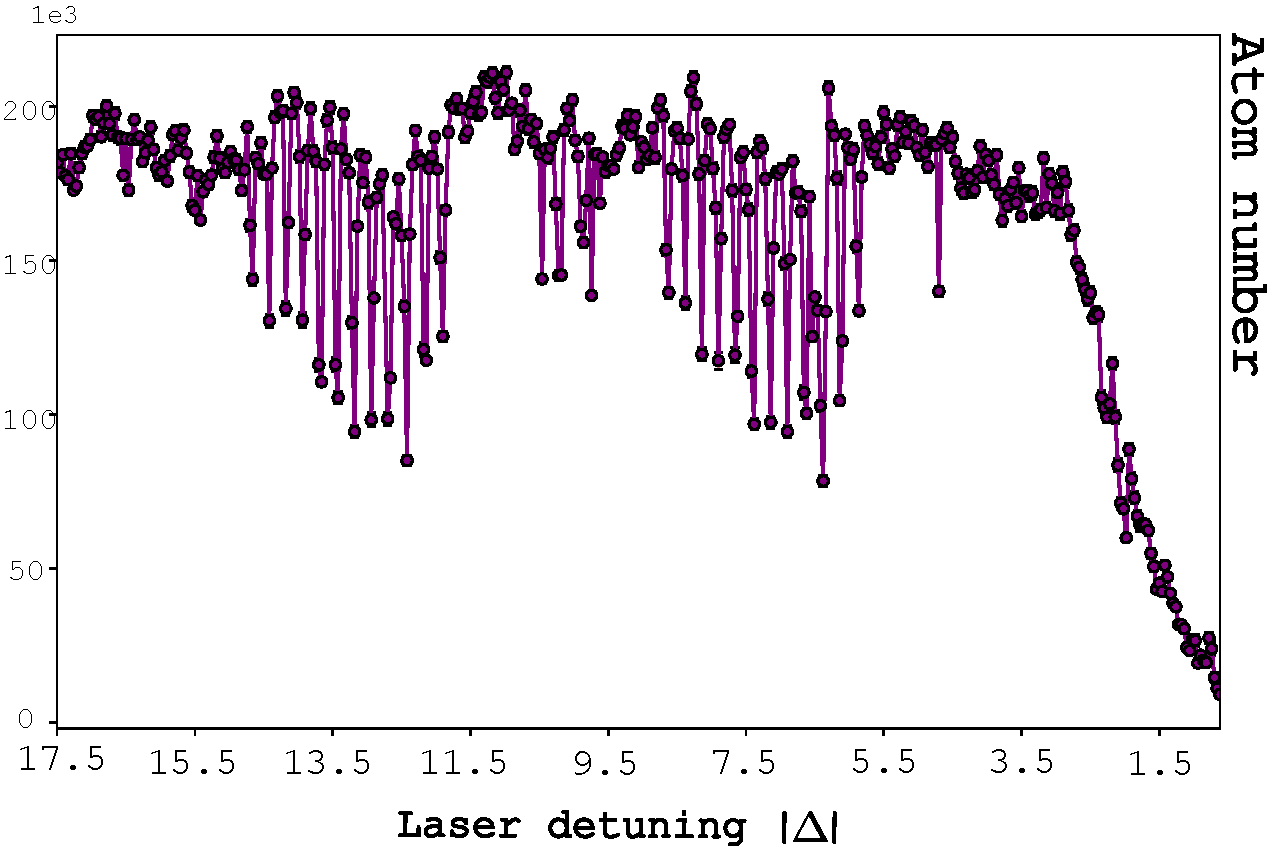
\includegraphics[width=0.49\linewidth, height=0.66\textheight, keepaspectratio]{87Sr/6MHz_blue_detuned.pdf}
\end{frame}

\end{document}
